% Copyright (c) 2022 Hans Wan, Chiro Liang and ReiSakuma
% All rights reserved.
% This paper is publicised for non-commercial learning purpose only.
% THIS PAPER IS PROVIDED ON AN "AS IS" BASIS, WITHOUT WARRANTIES OF ANY KIND,
% EITHER EXPRESS OR IMPLIED, INCLUDING BUT NOT LIMITED TO NON-INFRINGEMENT,
% MERCHANTABILITY OR FIT FOR A PARTICULAR PURPOSE.

\documentclass[a4paper]{article}
\usepackage{hcr-cumcm}
\usepackage[style=gb7714-2015,backend=biber]{biblatex}
\addbibresource{bibdata.bib}

\newcommand{\subsubsubsection}[1]{\paragraph{#1}\mbox{}\\}
\setcounter{secnumdepth}{4} % how many sectioning levels to assign numbers to
\setcounter{tocdepth}{4} % how many sectioning levels to show in ToC

\lstset{frame=tb,
%   language=Java,
  aboveskip=3mm,
  belowskip=3mm,
  showstringspaces=false,
  columns=flexible,
  basicstyle={\small\ttfamily},
%   numbers=none,
  numberstyle=\tiny\color{gray},
  keywordstyle=\color{blue},
  commentstyle=\color{dkgreen},
  stringstyle=\color{mauve},
  breaklines=true,
  breakatwhitespace=true,
  tabsize=2
}

\title{AquaFS 开发设计文档}

\begin{document}
    \pagestyle{plain}
    \maketitle

    %% ABSTRACT
    \section*{摘要}
\addcontentsline{toc}{section}{摘要}

ZenFS 由于其简单且与硬件 Zoned Storage SSD 紧密结合等特点,实现了零硬件预留空间、零硬件垃圾回收开销等高负载场景下的高性能特性,但是其仅适合 ZNS 设备、需要软件特殊适配等特点也限制了其应用场景灵活性。

AquaFS 是一个以 ZenFS 为原型的适用于 Zoned Storage SSD 的文件系统,将原来的 ZenFS 模块化,扩展其应用场景,添加 RAID 来平衡数据安全和写放大,同时添加调参模块以提高文件系统的智能性和性能。

在未来,我们将继续实现 AquaFS 的更多功能,如用户态 NVME 驱动加速、更完善的数据恢复、多文件系统融合调参等,进一步扩展应用场景并提升其智能化水平。

初赛阶段进度情况如表 \ref{progress} 所示。

\begin{table}[htbp]
  \centering
  \caption{初赛进度情况}
  \label{progress}
  \begin{tabular}{|l|l|p{8cm}|}
    \hline
    \textbf{改进内容}              & \textbf{完成进度} & \textbf{完成情况} \\
    \hline
    智能调参模块                   & 进度约70\%      & \checkmark 基于方差的重要参数选择方案 \\
                                  &                & \checkmark 基于高斯回归的调参方案 \\
                                  &                & $\square$ 将对垃圾回收参数进行进一步测试 \\
                                  &                & $\square$ 将对融合文件系统后的更多参数进行调优测试 \\
    \hline
    基于 Zone 的                  & 整体进度约 80\% & \checkmark 全盘 RAID 模式 RAID0、RAID1、RAID-C \\
    智能动态分区 RAID              &                & \checkmark 分区 RAID 模式 Zone 映射和 RAID 逻辑分配 \\
                                  &                & \checkmark 数据完整性检测和恢复 \\
    \hline
    异步 IO 优化                  & 进度约 60\%     & \checkmark 完成了 \verb|io_uring| 异步读写优化 \\
                                  &                & $\square$ 将进一步研究基于 spdk、xnvme 等的用户态 nvme 驱动 \\
    \hline
    融合通用文件系统               & 进度约 50\%     & \checkmark 基于 FUSE 和 Rust 完成一个 Ext2 兼容文件系统 \\
                                  &                & $\square$ 将进一步研究与 ZenFS 的结合方式 \\
    \hline
  \end{tabular}
\end{table}
    \tableofcontents
    %% CONTENT
    \section{概述}

本项目 AquaFS 是一个智能的 Flash 友好的文件系统,旨在为闪存设备提供更好的性能和更长的寿命。
本文档将从多个角度介绍 AquaFS 的设计与实现。

AquaFS 与传统文件系统相比,有以下几个特点:

\begin{itemize}
    \item 与 Ext4 等原地更新的文件系统不同,AquaFS 采用了日志结构,以减少写放大。
    \item 与传统软件文件系统不同,AquaFS 与硬件结合共同设计,降低硬件成本的同时提升性能。
    \item 与普通的单一文件系统不同,AquaFS 采用了多系统模块结合的方法,以提升系统的灵活性。
    \item 设计了专门的参数调整逻辑,以动态适应不同的工作负载。
    \item 设计了智能的读写逻辑,不同的工作负载能够由不同的模块处理或共同处理,以提升系统的性能。
    \item 优化垃圾回收逻辑,硬件上取消垃圾回收,软件上可调整预留空间与垃圾回收频率,以均衡调整性能与寿命。
    \item 其他特性。
\end{itemize}

后文将结合背景调研、需求分析、系统设计、系统实现、系统测试等方面,对 AquaFS 的各种设计特性进行详细介绍。

    \section{需求分析与调研}

\subsection{需求分析}

根据题目描述,我们需要实现一个“更加智能的 Flash 文件系统”。

Flash介质因本身的擦除特性,给上层文件系统带来与普通磁盘、内存文件系统不同的数据管理模式。
同时,Flash的写入放大、寿命以及后期稳定性下降等问题也给文件系统的设计带来的一定的挑战。
传统的Flash文件系统并没有很好地解决这些稳定性相关问题。
这里希望寻找一种更智能、更合适的Flash文件系统设计,来更好地平衡Flash的性能与稳定性。
可以思考的方向包括但不限于:数据压缩算法(可以是自适应的压缩算法),检错、纠错、纠删码(可以是联合信源信道编码),数据块选择、擦除策略,Cache机制。

结合赛题内容,我们需要完成的文件系统需要具备以下特性:

\begin{itemize}
  \item {\bf{适合 Flash 介质}}:文件系统需要能够适应并缓解 Flash 的写入放大、寿命、后期稳定性等诸多 Flash 存储介质特有的问题
  \item {\bf{更智能}}:文件系统需要使用多种策略,在软件算法层面平衡性能与寿命
\end{itemize}

\subsubsection{往年实现分析}

本题在去年已经有队伍选题并完成 \cite{youbifs-project},在选题之时,我们对前辈的项目进行了调研。

他们队伍完成了一个基于 UBIFS 的适用于裸 Flash 设备的 YOUBIFS 文件系统,从以下几个方面对其进行了优化:

\begin{itemize}
  \item {\bf{数据压缩模块}}:使用了预压缩和自适应压缩结合的方法,均衡压缩比和写入速度
  \item {\bf{纠错编码模块}}:实现自适应生命周期、CRC+RAID5两种纠错方案
  \item {\bf{Cache 机制}}:添加读写缓冲
  \item {\bf{冷热数据识别}}:使用了冷热识别的纠错以提高 I/O 速度
\end{itemize}

\begin{figure}[htbp]
  \centering
  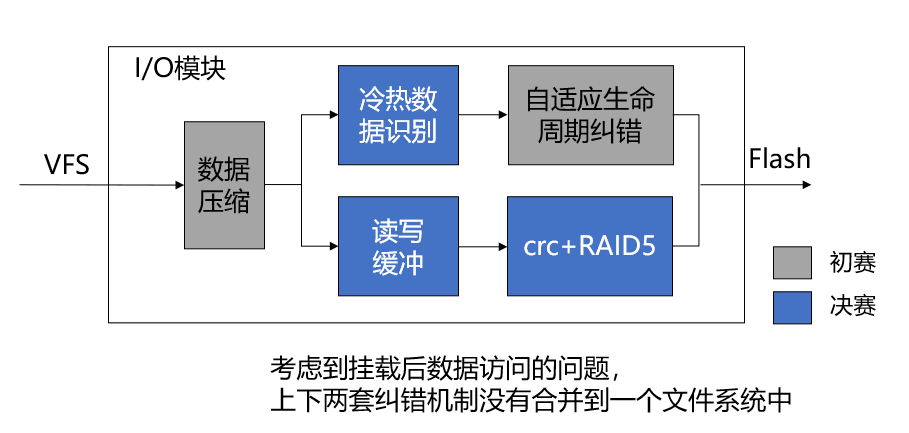
\includegraphics[width=0.7\textwidth]{fig/YOUBIFS项目框图}
  \caption{YOUBIFS 系统架构}
  \label{youbifs}
\end{figure}

YOUBIFS 的系统架构如图 \ref{youbifs} 所示。
看起来 YOUBIFS 的实现已经非常满足题目的需求,能够很好地回答题目中提出的几个问题。
但是我们发现,YOUBIFS 的系统实现也存在一些不足之处:

\begin{itemize}
  \item {\bf{Nor Flash 应用场景}}
    
  YOUBIFS 的实现中,文件系统的实现是针对于 Nor Flash 的。
  Nor Flash 在实现上与 Nand Flash 有很大的不同,因此 YOUBIFS 的实现并不能直接应用于 Nand Flash 上,应用场景受到了限制。
  
  同时,Nor Flash 一般用于嵌入式设备,而 Nand Flash 一般用于移动设备或高性能设备,因此 YOUBIFS 的实现也不能直接应用于移动设备或固态硬盘上。
  YOUBIFS 针对于 Nor Flash 的多种写入情况做了优化,但是由于 Nor Flash 的寿命、速度、稳定性等特性,其并不适合在写入负载较高的情况下工作。

  Nor Flash 的寿命一般在 10 万次左右,而 Nand Flash 的寿命一般在 100 万次左右\cite{cai_program_2013},因此 Nor Flash 广泛用于 BIOS 存储、固件存储等写入负载较低的场景。
  在这些应用场景下,由于存储的数据都是非常重要的系统关键数据,如 Bootloader、系统固件等,因此对于数据的稳定性要求非常高。
  如果系统软件直接在 Nor Flash 上频繁读写,很可能会导致 Nor Flash 的寿命过早耗尽,从而导致系统无法正常启动,造成非常严重的后果,
  所以 Nor Flash 很少用于存储程序运行过程中产生的数据,常见的写入场景为固件更新、系统升级等。

  因此,YOUFIBS 的实现并不能直接应用于移动设备或固态硬盘上,所针对的 Nor Flash 高压写入的应用场景也非常有限。
  这与 YOUBIFS 的各种优化策略相矛盾,因此我们需要重新设计一个适用于 Nand Flash 的文件系统,以扩展更多的应用场景。

  \item {\bf{“智能”,但是还不够智能}}

  YOUBIFS 的实现中,使用了多种策略来平衡性能与寿命,但是这些策略都是相对固定的,只是能够根据不同的情况进行策略切换。
  其中能够体现“智能”的实现有:

  \begin{enumerate}
    \item 通过判断文件名的方式来判断使用的压缩算法和参数,即压缩算法和等级的自适应
    \item 通过检查压缩效果是否合适来判断是否继续压缩,压缩效果不好可能其数据本身就是压缩文件,则再次不压缩
    \item 利用文件系统的 node,判别冷热数据文件
  \end{enumerate}

  为什么说我们认为这些“智能”策略其实还不够智能?
  
  这些策略的优化依据,都是文件系统的当前状态、当前负载请求分类等,没有充分考虑 Flash 的介质特性,如后期稳定性下降和延迟升高等,也没有充分考虑工作负载、实际应用和文件系统的互相配合。也就是说,考虑的因素还是不够多,对 Flash 的针对性优化也不够深入。

  同时,这些策略都是非常简单固定的逻辑。虽然通过参数上的调整,在性能受限制的嵌入式系统中也能够在指定的负载上取得比较好的效果,但是在性能限制不大、更复杂的系统中就很难有出色的表现。这是由策略本身的简单的性质决定的,复杂的系统往往需要更复杂的调整逻辑,而这就需要更加复杂的算法,从简单的逻辑判断到决策树、线性回归、神经网络等,用更加复杂和智能的策略逻辑来适应更加复杂的系统和更高要求的工作环境。

  \item {\bf{测试和展示不够规范}}

  首先是测试环境上的问题。录制的视频中的测试环境是个人计算机,目标设备是计算机上的 SSD 或者内存,而不是项目考虑中的 Nor Flash。

  既然是适用于 Flash 的文件系统,就应该统计和 Flash 相关的数据,从而衡量这个文件系统对 Flash 的稳定性、寿命、速度的综合影响,但是测试中只是在本机上进行了速度的测试,这难以说明问题。为了方便开发和开发过程中的验证,最好应该建立一个 Flash 仿真程序,真正计算在 Flash 中的读写频率、位置等信息,并模拟 Flash 芯片的具体延迟给出具体读写速度。

  其次,对 Flash 芯片的检错、纠错测试也应该基于 Flash 仿真,而不是在内存中写入值。在内存中改变一个或多个字节或比特,可能并不符合实际情况中的数据损坏场景。

  在决赛的文档中,记录了在实际嵌入式场景下在一个 Nor Flash 芯片上运行 YOUBIFS 的相关数据,但是没有体现在录制的展示视频中。演示视频中,不断切换测试脚本和开发环境,并通过切换分支的方式切换功能和版本。这样看视频的人很难看懂在做什么,看懂了也很难说明当前的设计有哪些提升。如果演示的时候就能直观地用自动化脚本生成测试报告,如表格、统计图等,会更加有表现力和说服力。
  没有使用通用的测试脚本或者软件,而是选择自己写脚本测试,难以说明提升。
  测试中大部分测试使用 3~11MiB 大小的连续读写,或者直接使用上百 MiB 的大文件连续读写,这不仅不能说明问题,而且也没有解决实际问题。在复杂的文件读写环境中,大部分读写应该是 4KiB 随机读写,这在其他的文件系统论文中是最重要的指标之一,视频中没有体现。

  \item {\bf{纠错算法和 UBIFS 本身不太兼容}}

  UBIFS 运行在 UBI 层之上,而 UBI 层本身已经做了一层校验和纠错,在上一层遇到一个两个比特级别的错误的可能性并不大,反而是一整块、一整个存储介质完全失效的可能性更高。而 UBIFS 本身的纠错算法是基于比特级别的,这样的纠错算法在 UBI 层已经做了纠错的情况下,就显得多余了。而且,UBIFS 的纠错算法是基于比特级别的,而 UBI 层的纠错算法是基于块级别的,这样的不兼容性也会导致 UBIFS 的纠错算法的效果不好。

  此外,YOUBIFS 中有 CRC+RAID5 的逻辑,但是其只适用于单个 Nor Flash 存储设备,在 UBI 层已经实现校验和纠错的情况下,基于 UBI 层的 YOUBIFS 更应该关注以块或设备为单位的 RAID,而不是以比特为单位的 CRC+RAID。

\end{itemize}

找出这些不足,我们并非为了挑刺,而是为了找到我们的项目前进的方向,摸着石头过河。除了这些不足之处,我们同样研究了前人项目的各种其他特点。

\begin{enumerate}
  \item {\bf{文档量很大:}} 文档中需要包含整个开发流程,需要列举并详细说明涉及到的技术要点和原理,以及配有丰富的示意图和代码段。在前人队伍的文档实现中,很大部分是分析原版 UBIFS 的实现逻辑和代码理解,另外一部分有基于这些理解对技术进行的调研以及自己的实现逻辑。  

  \item {\bf{总代码量很大:}} 原版 UBIFS 的代码量就有 1.5 MiB,所以对代码阅读理解能力也有很高的要求。去除重复文件后,使用 CLOC 统计文件行数如表 \ref{youbifs_code} 所示,队伍自己实现的部分暂未统计。

  \begin{table}
    \centering
  %   \begin{center}
      \begin{tabular}{lcccc}
        \textbf{Language} & \textbf{files} & \textbf{blank} & \textbf{comment} & \textbf{code} \\
        \hline
        C & 48 & 6044 & 12432 & 30124 \\
        C/C++ Header & 13 & 713 & 4033 & 4173 \\
        \hline
        SUM: & 61 & 6757 & 16465 & 34297 \\
      \end{tabular}
  %   \end{center}
      \caption{YOUBIFS 代码统计}
      \label{youbifs_code}
  \end{table}
  
\end{enumerate}

在 YOUBIFS 已经能够完成大部分题目要求的情况下,我们要如何在这个基础上进行改进呢?

依照上面的分析,首先我们可以改变我们文件系统的存储介质。YOUBIFS 使用的是 Nor Flash,那么我们可以选择 Flash 的另一种更加常用更加高性能的品类:Nand Flash。我们的研究基于 Nand Flash,就可以更加贴近实际应用场景,扩展项目的实际用途,也可以更加容易地和其他的文件系统进行对比。

其次,当我们选择了 Nand Flash,就多了一个技术实现上的选择。在许多较为低端的嵌入式设备上,主控是直接控制存储设备的绝对地址的。在 Linux Kernel 中,这样直接控制地址的设备被称为 MTD 设备(Memory Technology Device)。
除了 MTD 设备,还有一种方式是硬件层面实现一个从逻辑地址到绝对地址的映射,从而完成磨损均衡、垃圾回收等功能。这一层转换层叫做 FTL(Flash Translation Layer,FLash 地址转换层),在许多消费级、商业级服务器或者高端嵌入式设备上都会使用 FTL。在 Linux Kernel 中,这样的设备往往分类为块设备,而不是 MTD 设备。

\begin{figure}[htbp]
  \centering
  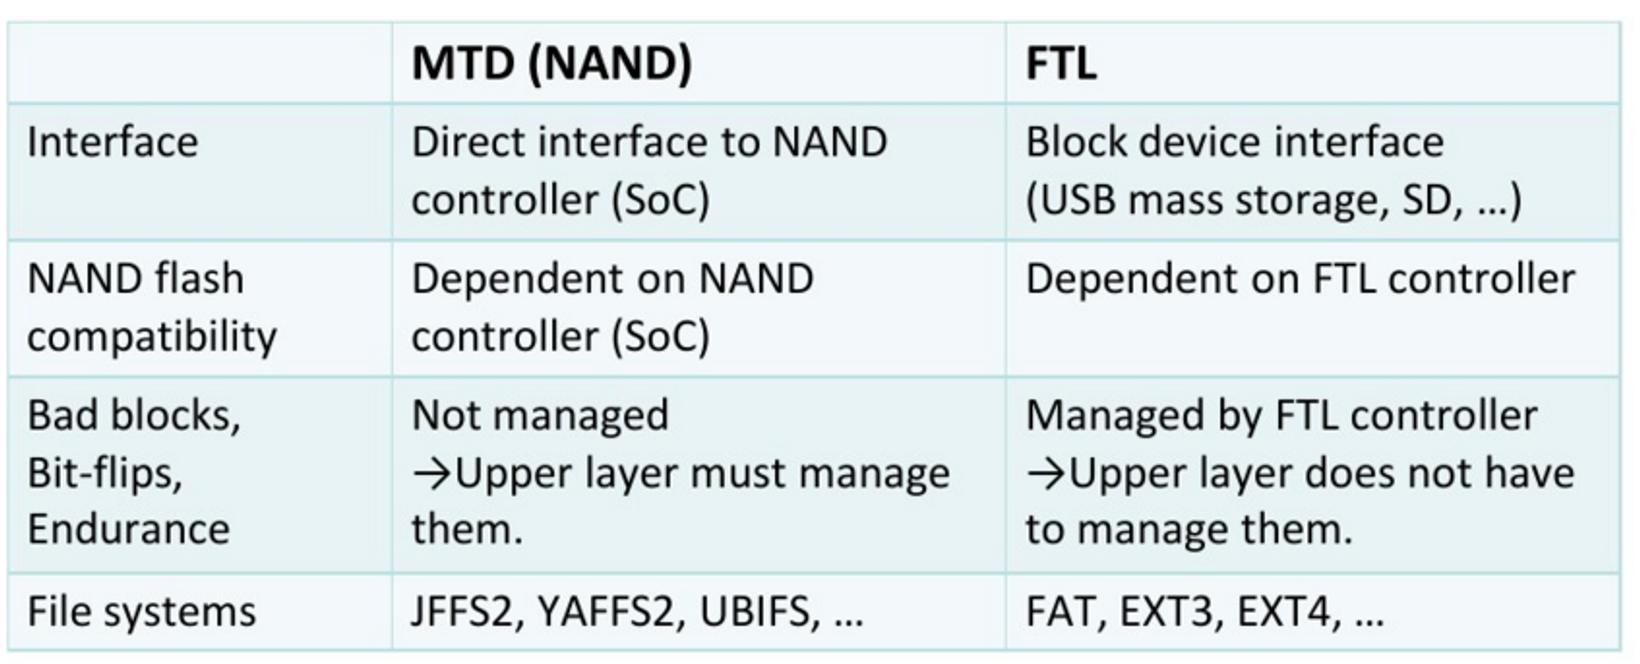
\includegraphics[width=0.7\textwidth]{fig/flash-mtd-ftl}
  \caption{MTD 设备和有 FTL 的设备的对比}
  \label{flash-mtd-ftl}
\end{figure}

MTD 设备和有 FTL 的设备的对比如图 \ref{flash-mtd-ftl} 所示。在我们的项目中,我们选择了基于 Nand Flash 的块设备,而不是基于 Nand Flash 的 MTD 设备,这样可以更加贴近实际应用场景,扩展项目的实际用途,也可以更加容易地和其他的文件系统进行对比。

我们选择基于 Nand Flash 与 FTL 的文件系统,题目需求中的许多方面都出现了新的需求。首先,Nand Flash 的读写单位是页,而 Nor Flash 的读写单位是字节,这就要求我们的文件系统在读写时要考虑到页的边界对齐问题。其次,Nand Flash 之上的一层 FTL,向上隔绝了数据块选择、数据擦除、逻辑物理地址映射等与 Flash 存储介质相关的细节,从而提高了在文件系统层面针对 Flash 进行优化的难度。最后,Nand Flash 的读写速度比 Nor Flash 快,但是擦除速度比 Nor Flash 慢,这就要求我们的文件系统在设计时要考虑到这一点,尽量减少擦除操作的次数。

为了解决这些问题,我们需要对 Nand Flash 的特性进行调研,然后在一种基于 Nand Flash 的文件系统的基础上进行改进。

\subsection{背景调研}

在我们选定赛题后,我们立刻开始了针对 Flash 文件系统实现的调研。

\subsubsection{Flash 的特点和分类}

为了实现针对 Flash 优化的文件系统,我们必须首先了解 Flash 的各种特性和分类。

闪存(Flash Memory)是由日本的 舛岡富士雄 (Fujio Muoka)发明的。他分别于1966年和1971年从日本东北大学(Tohoku University)获得学士和博士学位,博士毕业之后他加入了东芝(Toshiba)公司。在东芝工作期间,他分别于1980年和1988年发明了NOR Flash 和 Nand Flash。

目前市面上的闪存主要有两种:NOR Flash 和 Nand Flash,其分类逻辑和原理如图 \ref {flash-nand-nor} 所示。
一般而言,并行接口的Parallel Flash是基于NOR Flash的;而SSD硬盘,U盘,SD卡,eMMC等通常是基于Nand Flash的。

\begin{figure}[htbp]
  \centering
  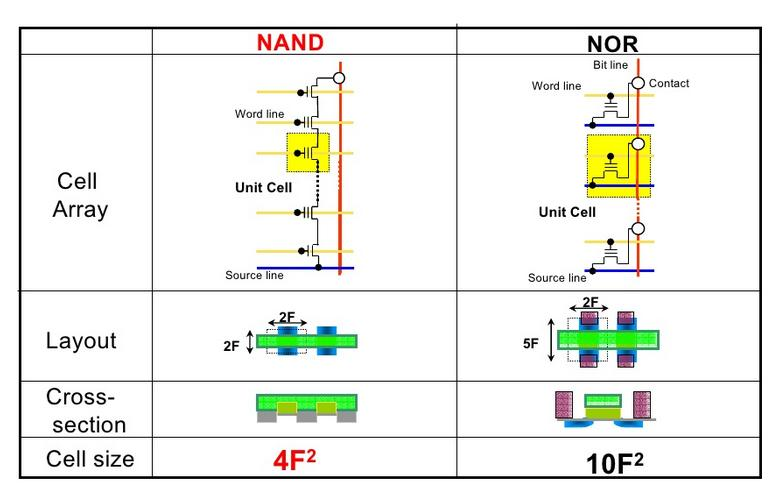
\includegraphics[width=0.85\textwidth]{fig/flash-nand-nor}
  \caption{Flash 原理与分类}
  \label{flash-nand-nor}
\end{figure}

\subsubsection{Nand Flash}
\label{flash-nand}

Nand Flash 是一种非易失性存储器,具有访问速度快、存储密度高、成本低的特点。Nand Flash 的读写操作都是以页为单位进行的,而且每次写操作都需要先擦除整个块,这使得 Nand Flash 更适合用于存储大量数据,而不适合用于执行代码和固件更新等应用。然而,Nand Flash 的读写速度快,成本低,是目前大多数嵌入式设备或消费级、商业级电子产品的主要存储介质。

\begin{figure}[htbp]
  \centering
  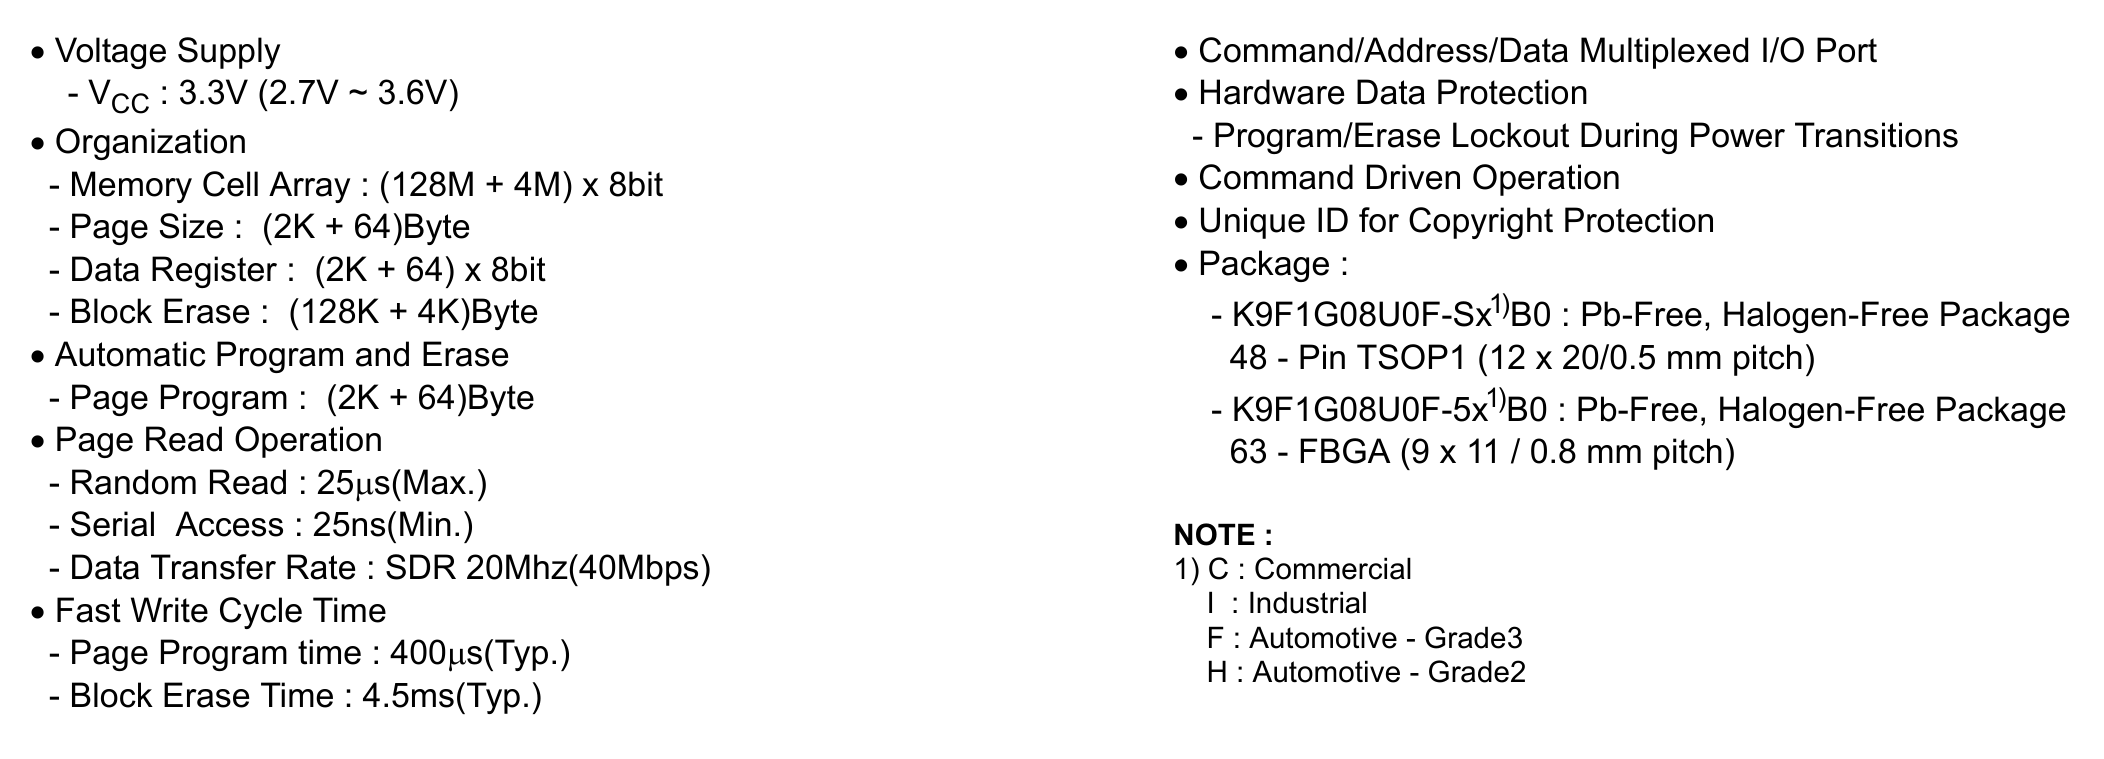
\includegraphics[width=0.85\textwidth]{fig/flash-nand-feature}
  \caption{K9F1G08U0F-5IB0 特性}
  \label{flash-nand-feature}
\end{figure}

为了详细了解 Nand Flash 的多种特性,我们专门针对一款常用的 Nand Flash 进行了调研。这款 Nand Flash 的型号是 K9F1G08U0F-5IB0。这是一款来自三星的 SLC Nand,容量为 1Gb,其主要特性如图 \ref{flash-nand-feature} 所示。

在读写操作失败时,Nand 控制器需要进行一些特殊的处理。将 Datasheet 中的处理方式翻译为中文:在 NAND Flash 存储器中,其使用寿命内可能会出现额外的无效块。请参考资格报告以获取实际数据。应考虑以下可能的故障模式以实现高度可靠的系统。在擦除或编程后状态读取失败的情况下,应进行块替换。因为在页面编程期间的编程状态失败不会影响同一块中其他页面的数据,所以可以通过找到一个已擦除的空块,并重新编程当前目标数据并复制替换块的其余部分,来执行块替换。在读取时必须使用 ECC。为了提高内存空间的效率,建议通过 ECC 回收由于单个位错误而导致的读取或验证失败,而无需进行任何块替换。所述附加块故障率不包括那些被回收的块。写入时错误处理流程如图 \ref{nand-rw-err} 所示。

\begin{figure}[htbp]
  \centering
  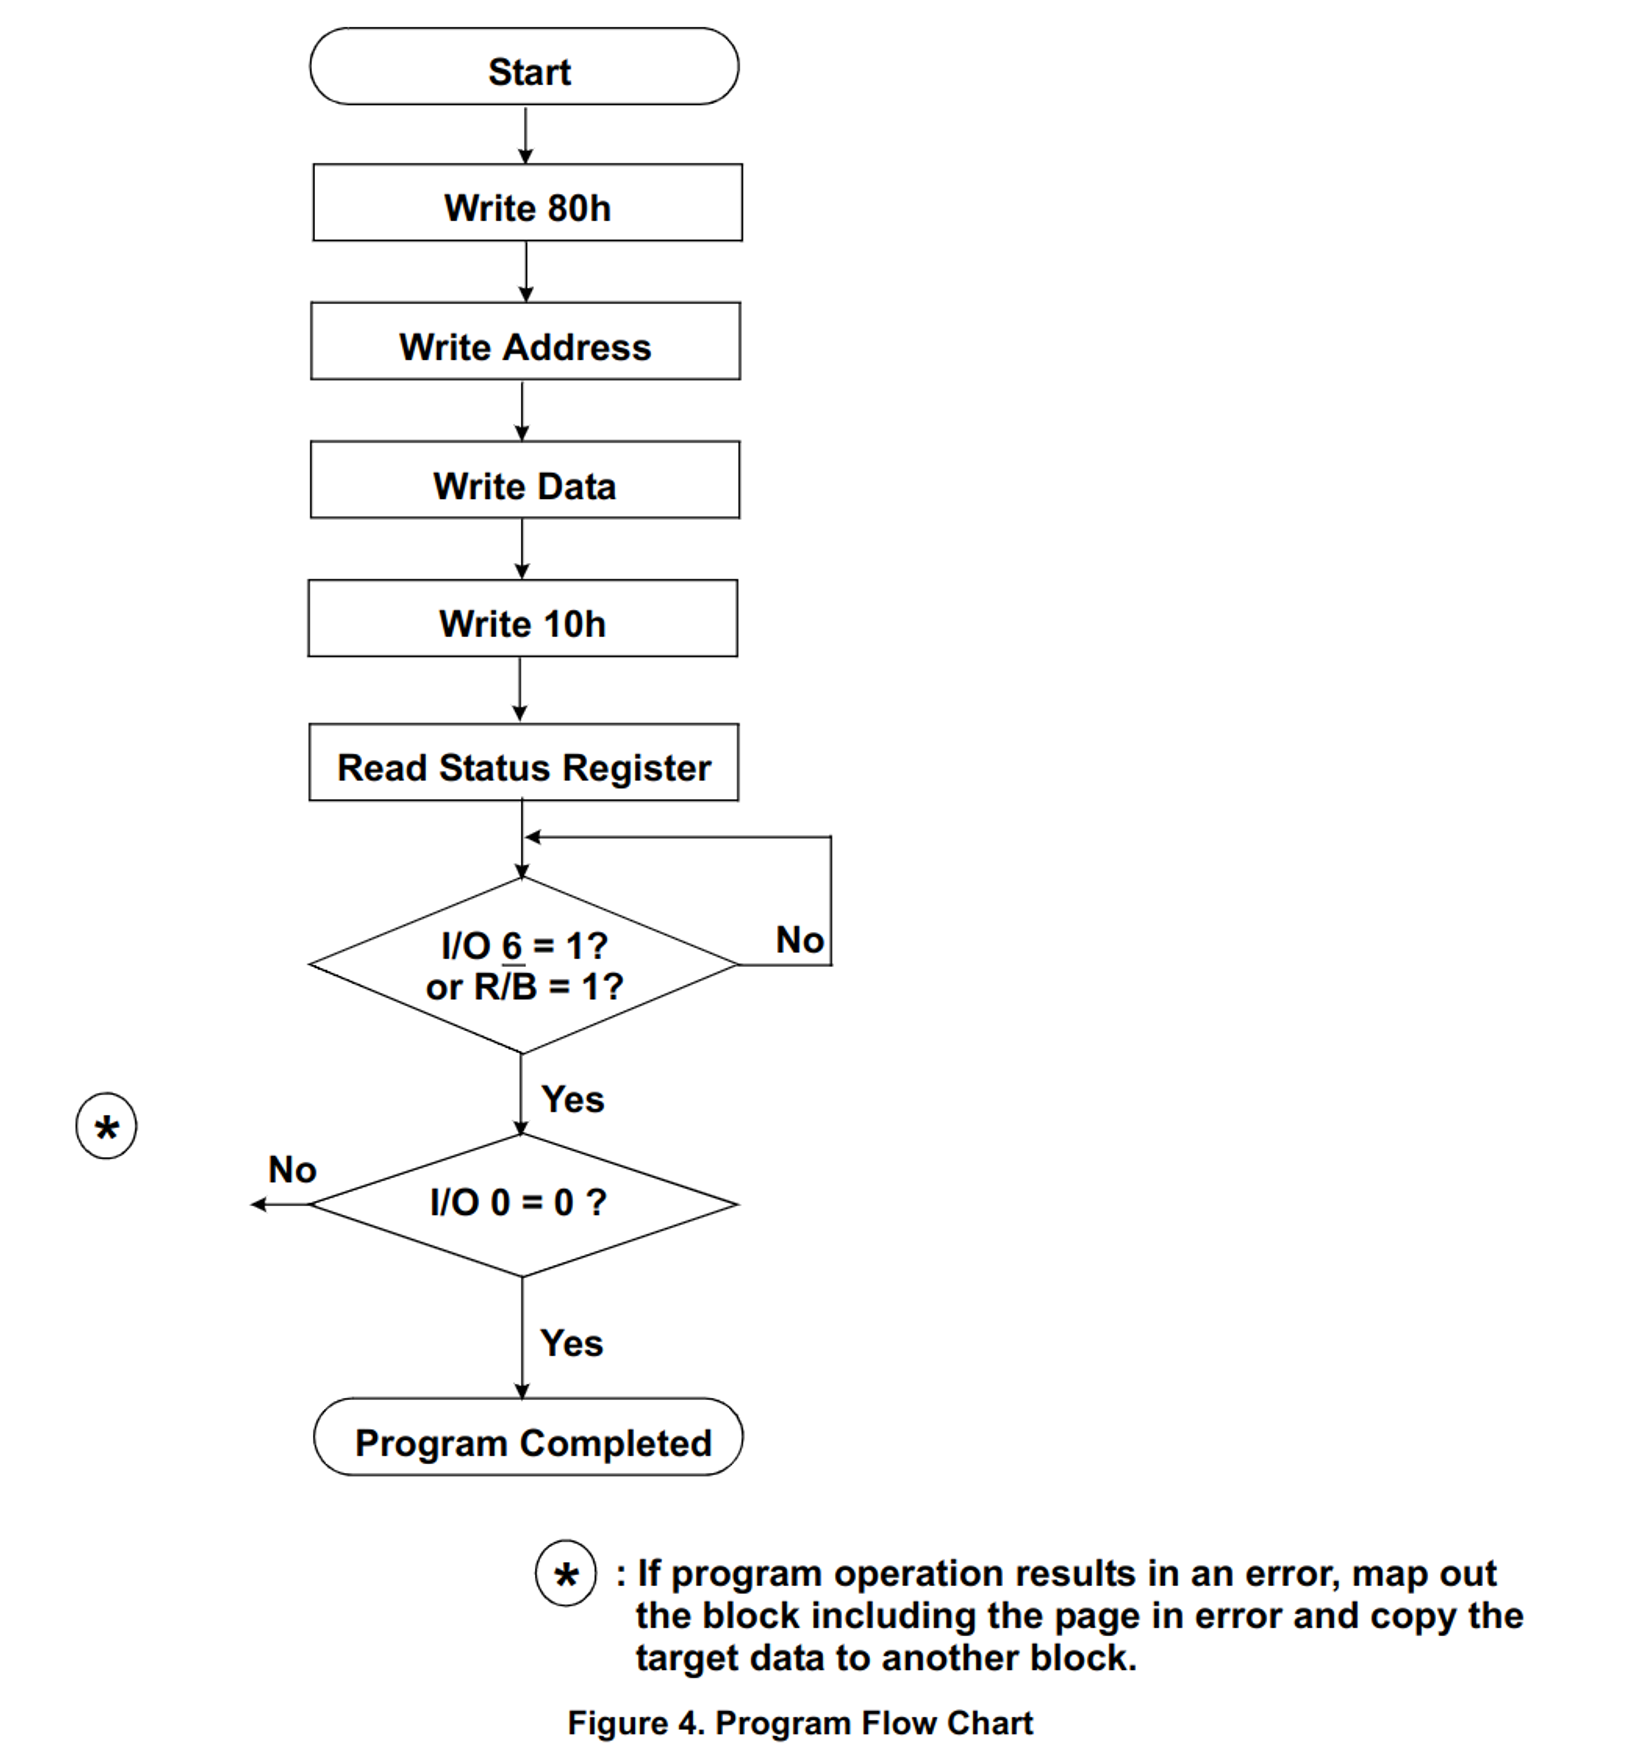
\includegraphics[width=0.85\textwidth]{fig/nand-rw-err}
  \caption{写入时错误处理流程}
  \label{nand-rw-err}
\end{figure}

Nand 由于其以页面为写入单位的特性,使得其在写入时的错误处理流程较为复杂。在写入时,如果发生错误,需要进行块替换。块替换的过程如图 \ref{nand-replace} 所示。

\begin{figure}[htbp]
  \centering
  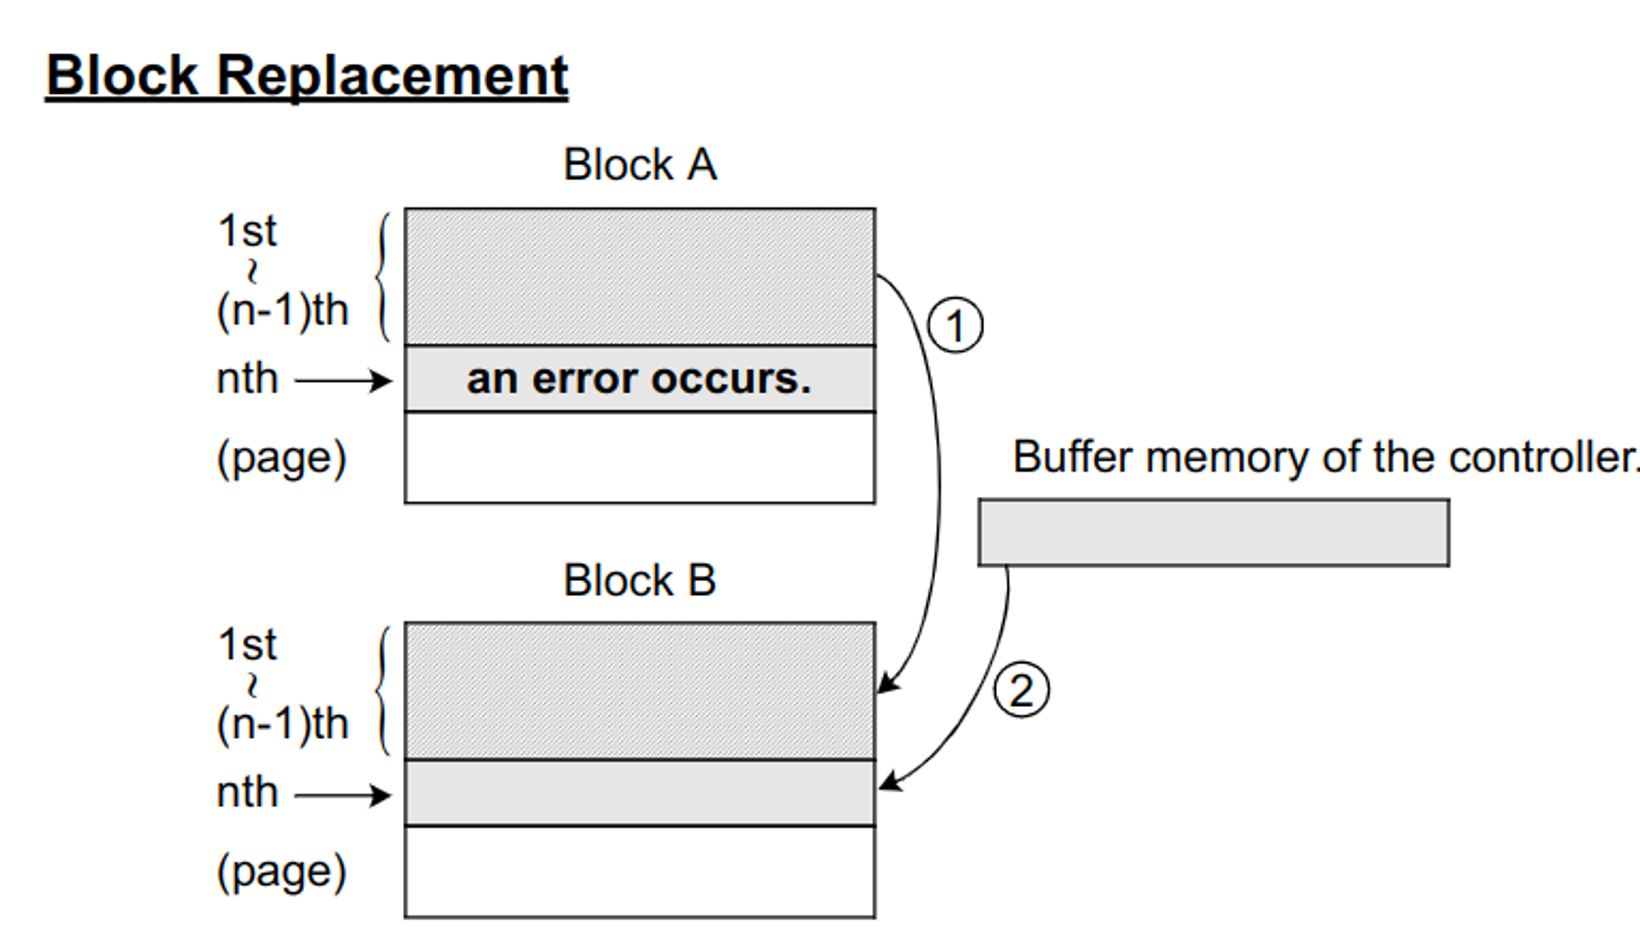
\includegraphics[width=0.85\textwidth]{fig/nand-replace}
  \caption{Nand 块替换流程}
  \label{nand-replace}
\end{figure}

由于 Nand Flash 只能以页面为单位进行写入,所以在一个块内,页面必须从该块的LSB(最低有效位)页面到该块的MSB(最高有效位)页面依次编程,禁止随机页面地址编程。在这种情况下,LSB页面的定义是要编程的页面中的LSB。因此,LSB不需要是页面0。

\begin{figure}[htbp]
  \centering
  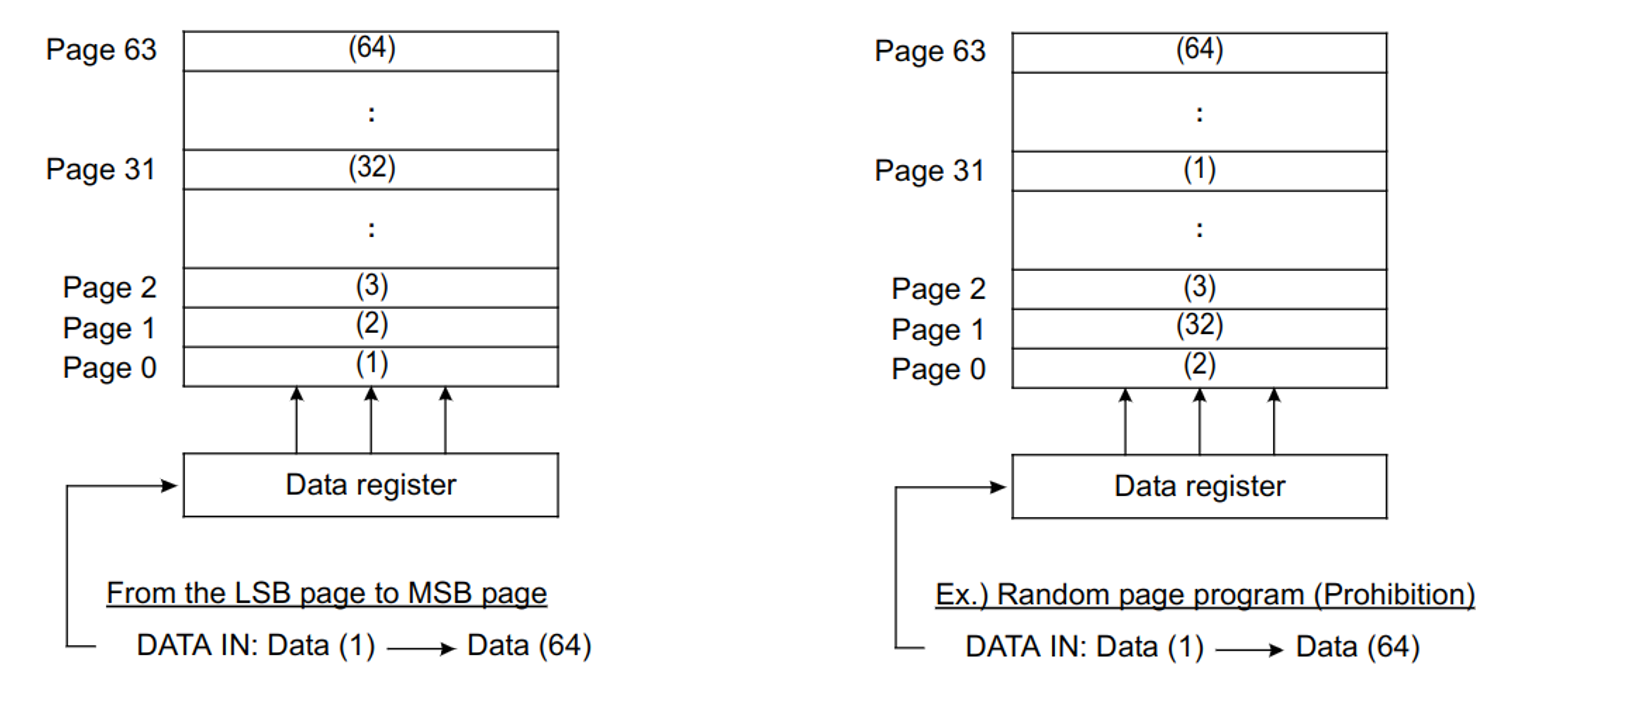
\includegraphics[width=0.85\textwidth]{fig/nand-write-addr}
  \caption{Nand 写入寻址举例}
  \label{nand-write-addr}
\end{figure}

这个用于举例的 Flash 芯片已带有 ECC 功能。在编程操作期间,内部ECC逻辑生成ECC。在读取操作期间,设备会自动执行ECC。读取操作执行后,可以发出读取状态命令以识别读取状态,读取状态保持不变,直到执行其他有效命令。这个 Nand Flash 可以自己纠正 4bit 的错误。

即,这款 Nand 芯片内的控制器能够保证在读取时,能够自动执行 ECC,并且能够自动纠正 4bit 的错误。这样,我们在读取时,基本不需要考虑较少比特位的 ECC 的问题。当 Nand 芯片内的控制器检测到无法纠正的 ECC 错误,将会返回错误信息,然后可以根据这个错误信息,进行块替换。如果块替换失败,那么这个块就会被标记为坏块,不再使用。

由此得知,一般 Nand 芯片向外提供的数据接口可以保证数据的正确性,从而上层软硬件可以依赖于 Nand 上的硬件 ECC 提供的数据正确性保证。但是这是在 Nand 使能了 ECC 功能的情况下,如果 Nand 芯片没有使能 ECC 功能,那么上层软硬件就需要自己实现 ECC 算法,来保证数据的正确性。此外,硬件 ECC 功能需要占用额外的磁盘空间,因此,如果对磁盘空间有较高要求,那么可以考虑不使能硬件 ECC 功能。

\subsubsection{Nor Flash}

NorFlash 是一种非易失性存储器,具有访问速度快、读写寿命长、可靠性高的特点。与 Nand Flash 不同,NorFlash 的读操作可以以随机方式进行,而不需要预先擦除整个块。这使得 NorFlash 更适合用于执行代码和固件更新等应用,可以加速启动时间和提高系统性能。然而,NorFlash 的密度较低,成本较高,不适合用于存储大量数据。

NorFlash 的一些其他特点包括:

\begin{itemize}
  \item {\bf{高度可靠}}:Nor Flash 可以实现数据的可靠存储和读取,并且具有高度可靠性。
  \item {\bf{可以执行代码}}:Nor Flash 可以作为代码存储器,可以加快启动时间并提高系统性能。此外,Nor Flash 还支持 XIP(执行内存),它允许 CPU 直接从 Nor Flash 中执行代码,而无需将代码加载到 RAM 中。
  \item {\bf{读写寿命}}:Nor Flash 的读写寿命比 Nand Flash 长得多,因此它更适合于需要高度可靠性和长寿命的应用程序。
  \item {\bf{错误概率}}:Nor Flash 读写操作的错误概率很低,这使得它在数据存储和传输方面更加可靠。
\end{itemize}

\subsubsection*{Nand flash 和 Nor flash 的性能比较}

flash闪存是非易失存储器,可以对称为块的存储器单元块进行擦写和再编程。任何flash器件的写入操作只能在空或已擦除的单元内进行,所以大多数情况下,在进行写入操作之前必须先执行擦除。NAND器件执行擦除操作是十分简单的,而NOR则要求在进行擦除前先要将目标块内所有的位都写为0。由于擦除NOR器件时是以64~128KB的块进行的,执行一个写入/擦除操作的时间为5s,与此相反,擦除NAND器件是以8~32KB的块进行的,执行相同的操作最多只需要4ms。执行擦除时块尺寸的不同进一步拉大了NOR和NADN之间的性能差距,统计表明,对于给定的一套写入操作(尤其是更新小文件时),更多的擦除操作必须在基于NOR的单元中进行。

Nand Flash 与 Nor Flash 的主要区别如下:

\begin{itemize}
  \item NOR的读速度比NAND稍快一些。
  \item NAND的写入速度比NOR快很多。
  \item NAND的4ms擦除速度远比NOR的5s快。
  \item 大多数写入操作需要先进行擦除操作。
  \item NAND的擦除单元更小,相应的擦除电路更少。
\end{itemize}

我们最终选定了 Nand Flash 作为我们的存储介质,主要是因为 Nand Flash 的价格更低,而且 Nand Flash 的读写速度更快,更适合于我们的应用场景,同时与其他赛组的工作能保持一定的区分度。

\subsubsection{FTL}

FTL(Flash Translation Layer,闪存地址翻译层)是广泛存在于 Nand Flash 存储层次之上的一层地址翻译逻辑,它的主要作用是将逻辑地址转换为物理地址。

FTL 通常是由 Nand Flash 的厂商提供的,因此,不同厂商的 FTL 实现可能会有所不同,但是它们的主要功能都是相同的,即地址映射。原因是闪存只能异地更新,为了对上支持数据块原地更新则需要通过地址转换实现。由于闪存先擦后写、擦写有次数限制(寿命)、使用过程中会不断出现坏块(块寿命不同)等特性,FTL还需具备垃圾回收、磨损均衡、坏块管理等十八般武艺。

闪存内部的基本存储单位是Page(4KB),N个Page组成一个Block。FTL 的映射方式主要有:

\begin{enumerate}

  \item \textbf{块级映射}

  将块映射地址分为两部分:块地址和块内偏移。映射表只保存块的映射关系,块内偏移直接对应。

  \item \textbf{页级映射}

  映射表维护每个页的映射关系。

  \item \textbf{混合映射}

  主要思路是针对频繁更新的数据采用页级映射,很少更新的数据采用块级映射。其中采用Log Structured思想的混合映射将存储分为数据块(Data Block)和日志块(Log Block)。数据块用于存储数据,采用块级映射,日志块用于存储对于数据块更新后的数据,采用页级映射。混合映射是低端SSD、eMMC、UFS广泛采用的映射方式。根据日志块和数据块的对应关系又可以分为全相关映射(FAST)、块相关映射(BAST)、组相关映射(SAST)等等。下图是SAST映射的一个示例:2个日志块对应4个数据块,当日志块用完时需要通过搬移有效数据回收日志块。对于顺序写场景,最好情况下日志块对应位置记录了数据块的更新,则可以无需搬移数据,直接将日志块作为新的数据块,数据块进行擦除操作作为新的日志块。对于大量随机写场景,则需要将日志块和数据块中的有效数据搬移到空闲块的对应位置作为新的数据块,然后擦除原日志块和数据块。

\end{enumerate}

由于 FTL 一般实现在 SSD/EMMC 主控中,作为一个黑盒存在,因此上层软件无法得知 FTL 的具体实现,也无法对其进行优化。举个例子,如果上层软件知道 FTL 的映射方式是页级映射,那么它就可以将多个小文件合并成一个大文件,这样就可以减少 FTL 的映射表的大小,从而提高性能。但是上层软件往往并不知道 FTL 的映射级别和映射表的大小,因此无法进行优化;如果软件贸然进行优化,反而可能会触发 FTL 的垃圾回收机制等,从而造成更大的写放大和性能降低。

此外,FTL 的映射逻辑需要占用一定的存储空间,这也是 FTL 的一个缺点。加上主控的垃圾回收功能,一款 SSD 往往有 10\% 到 20\% 的空间是不可用的,这也是 SSD 的一个缺点。

\subsubsection{SSD 的性能瓶颈}

SSD 的性能瓶颈涉及多个方面:

首先,闪存芯片本身的读取和写入速度是一个重要的性能瓶颈。尽管闪存技术不断进步,但相对于传统的机械硬盘,闪存的读取和写入速度仍然有限。特别是对于随机的小块读写操作,闪存的延迟和响应时间可能较高。

其次,闪存芯片的擦写操作是一项耗时的操作,因为擦除一个块通常需要先将其数据复制到其他位置,然后进行擦除操作。这导致了写入操作的额外开销和延迟,尤其在频繁的写入场景下,擦写操作的成本会进一步增加。

另外,闪存芯片的寿命限制也是一个性能瓶颈。闪存芯片具有有限的擦写次数,每次擦写操作都会减少芯片的寿命。当某些块的擦写次数达到上限时,需要进行垃圾回收和数据迁移操作,这可能导致额外的延迟和性能损耗。

存储控制器也对SSD的性能起着重要作用。存储控制器负责管理闪存芯片、处理IO请求、执行错误校验和纠正(ECC)等功能。较低性能的存储控制器可能成为整个系统的瓶颈,限制了SSD的性能表现。

最后,接口和总线的带宽限制也可能影响SSD的性能。常见的接口如SATA、PCIe、NVME等,其带宽和传输速度对于数据的读取和写入速度有一定影响。如果接口和总线的带宽无法满足SSD的性能要求,可能会限制SSD的吞吐量和响应时间。

我们选定了需要做基于 Nand Flash 的文件系统,就必须要直面以上的问题,我们需要在文件系统层面上解决这些问题,使得文件系统能够更好的利用 Nand Flash 的特性,提高文件系统的性能。

经过调研,我们发现了许多现有的基于 Nand Flash 的文件系统,如 Btrfs、LogFS、F2FS 等。这些文件系统都是为了解决 Nand Flash 的特性而设计的,它们都有各自的优缺点,但是都是在当下已经有完善的 FTL 映射的情况下去解决这个问题。

如果有一种“文件系统”,能够在上层软件和下层硬件之间沟通协调,让软硬件各自更加各司其职,做更适合做的事情,那么能不能解决上面提到的诸多困难呢?

于是乎,我们找到了 ZenFS。这是一个简单的“文件系统”,但是它却能够做到保持最高性能写入不掉速,能做到 100\% 的空间利用率,能做到最高的数据库随机读写速度和最低的读写延迟。对这样一种“文件系统”,我们立刻产生了极大的兴趣。对 ZenFS 的调研,详见第 \ref{chap:zenfs} 章的介绍。

\subsubsection{文件系统调参}

在数据库和文件系统这些存储系统中中实现良好的性能并非易事,因为它们是复杂的系统,具有许多可调选项,这些选项几乎控制其运行时操作的许多方面。在这些系统中,配置参数是一个重要的问题。存储系统通常有许多影响其行为的参数,调整这些参数可以显着提高性能。由于大量的参数和可能的配置呈指数级增长,手动和自动调整方法都很费力。

鉴于此,许多组织会聘请昂贵的专家来配置系统的参数。但是随着应用程序在规模和复杂性方面的增长,优化参数以满足应用程序的需求已经超越了人类的能力。这是因为参数的正确配置在很大程度上取决于许多人所无法推理的因素。

于是,我们预期实现一个智能调参模块来使得作为RocksDB插件的文件系统AquaFS具有自动调整本身参数的能力,以使得文件系统更加智能,减少可能的人力开销。

在智能调参方面主要设计到两个方面,参数选择和参数调整。

在参数选择方面,存储系统通常有许多影响其行为的参数。存储系统是现代计算机系统的关键组件,对应用程序性能和效率有重大影响。大多数存储系统都有许多可配置的参数来控制和影响它们的整体行为。例如,Linux 的Ext4提供了大约60个参数 \cite{ext4doc},代表超过 1037种潜在的配置状态。默认设置通常不是最优的;有研究表明,调整存储参数可以将系统性能提高多达 9倍 \cite{Sehgal2010EvaluatingPA}。

为了应对大量可能的配置,系统管理员通常专注于使用他们的领域专业知识来调整一些经常使用和经过充分研究的参数,这些参数被认为会显着影响系统性能。然而,面对日益增加的复杂性,这种手动调整方法并不能很好地扩展。现代存储系统使用不同的文件系统类型(EXT4,XFS,Btrfs)、新硬件(SSD、SMR、NVM)、多层和混合存储,和多个虚拟化层(例如 LVM、RAID)。存储系统范围从一个或几个相同的节点到数百个高度异构的节点在参数调整方面。

最近,已存在多种优化方法来自动调整存储系统,在合理的时间范围内实现了良好的性能改进\cite{10.5555/3277355.3277441,10.1145/3545008.3545012}。这些自动调整技术将存储系统建模为黑匣子,反复尝试不同的配置,测量目标函数的值,并根据先前学习的信息选择新的配置进行尝试。然而,许多黑盒自动调整技术难以扩展到高维,并且可能需要很长时间才能收敛到好的解决方案。因此,处理大量存储参数配置的问题在很大程度上仍未解决。

在机器学习和信息论中,降维是处理大型数据集的常用技术。如果它可以应用于存储系统,它将大大减少搜索空间,使人类或算法更容易调整存储系统。以前的研究中提到,并非所有存储参数都具有同样重要的性能影响:一些参数比其他参数具有更大的影响 \cite{10.5555/3277355.3277441}。这自然促使我们研究如何量化每个存储参数的影响或重要性,以及如何有效地选择重要参数。

现在存在许多方法来解决维数灾难的问题,也即降维方法。降维方法通常可以概括为两类:特征提取和特征选择。

特征提取是指将高维数据投影到低维空间;新构建的特征通常是原始特征的线性或非线性组合。常见的特征提取方法包括主成分分析 (PCA)、独立成分分析和线性判别分析。特征提取的一个主要缺点是每个特征的物理意义都会因投影和许多维度的非线性组合而丢失。因此,常见的特征提取技术与本文中的目标相冲突:即选择一些可以理解和解释的原始存储参数。

相反,特征选择直接从原始特征中选择一个特征子集,目的是只找到重要的特征。特征选择方法可以分为监督或非监督方法。无监督特征选择,例如 Principle Feature Analysis ,根据特征之间的关系选择包含大部分基本信息的子集。在选择阶段不考虑特征对优化目标的影响。相反,有监督的特征选择选择一个可以区分或近似目标变量的子集。其中包括基于决策树的算法等等。由于我们有兴趣找到对我们的优化目标有重大影响的参数,例如 I/O 吞吐量,因此监督特征选择最适合我们的需求 \cite{mahmud_confd_nodate}。

由于在存储系统中存在许多离散的参数,将这些离散参数抽象成离散值的质量决定了特征选择的质量,将具有 N 个值的分类参数转换为 N 个单独的二进制参数会使参数空间呈指数级扩展。因此本文并没有采用lasso回归,lasso回归的计算成本很高。

另一种流行的特征选择方法是建立在信息论的基础上的方法。这些方法通常为某些子集中目标变量的同质性定义一个度量。常用的指标包括连续变量的方差等。在本文中,们采用基于方差的重要参数选择方案,方差在系统中的对比可以凸显出参数的重要性。

在参数调整方面,是对于参数选择中的重要参数进行参数的调整。

在之前的对数据库进行自动调参的研究中 \cite{10.1145/3035918.3064029},对数据库的表征负载进行提取,在匹配了相似负载,并用lasso回归对参数进行去冗余降维之后,采用了高斯过程回归的方案进行参数的调整。高斯过程回归是一种先进的技术,其功能与深度网络的功能大致相当。高斯过程回归有许多吸引人的特性,使其成为配置空间建模和提出建议的合适选择。最重要的是,一个是高斯过程回归默认提供置信区间。在该研究中采用了两种方案提供推荐的参数,其中一种是直接匹配相似负载中的最好配置,另外一种是尝试回归的配置。本文中尝试使用两种方案。

\subsection{ZenFS}
\label{chap:zenfs}

\subsubsection{ZenFS 的特点}

ZenFS 是一个 RocksDB 的文件系统插件,它利用 RocksDB 的文件系统接口将文件放置到原始分区块设备上的区域中。通过将文件分成多个区域并利用写入生命周期提示来共同定位具有相似生命周期的数据,与传统的块设备相比,系统写入放大大大降低了。 ZenFS 确保文件系统或磁盘上没有后台垃圾收集,从而提高吞吐量、尾部延迟和磁盘耐久性方面的性能(图 \ref{zns-write})。ZenFS 的整体架构如图 \ref{zenfs-overview} 所示。\cite{bjorling_zns_nodate}

\begin{figure}[htbp]
    \centering
    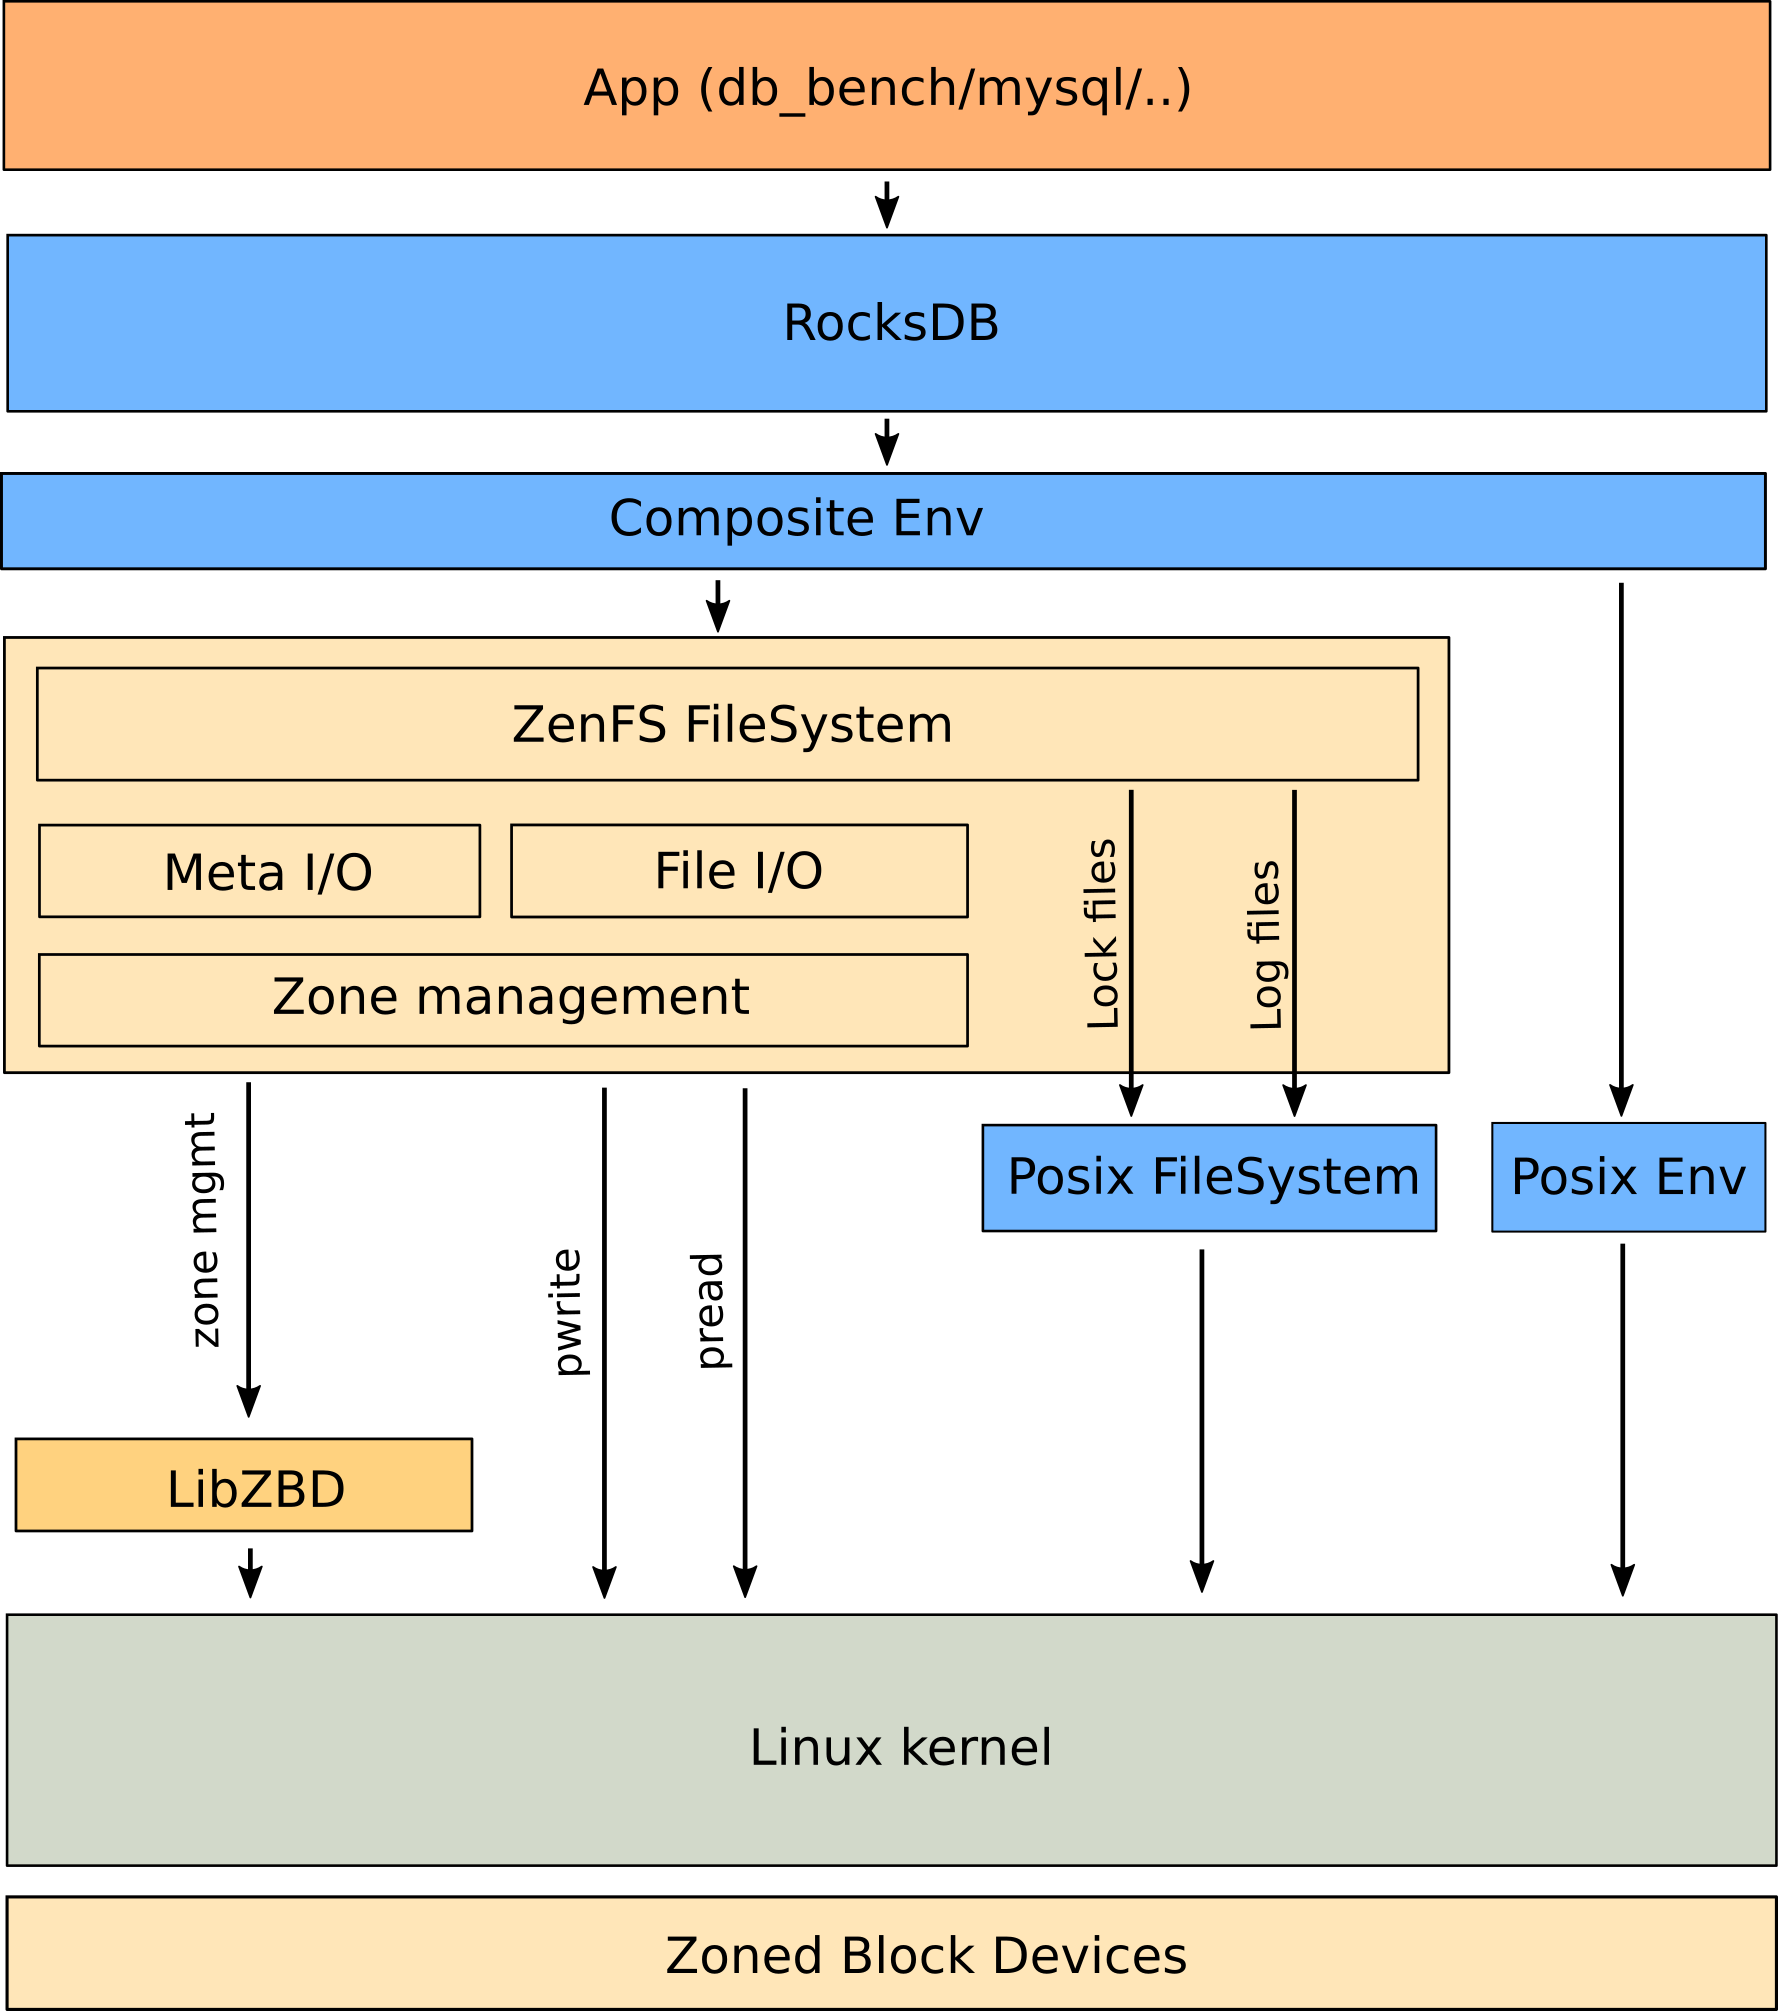
\includegraphics[width=0.8\textwidth]{fig/zenfs-overview}
    \caption{ZenFS 架构}
    \label{zenfs-overview}
\end{figure}

\begin{figure}[htbp]
    \centering
    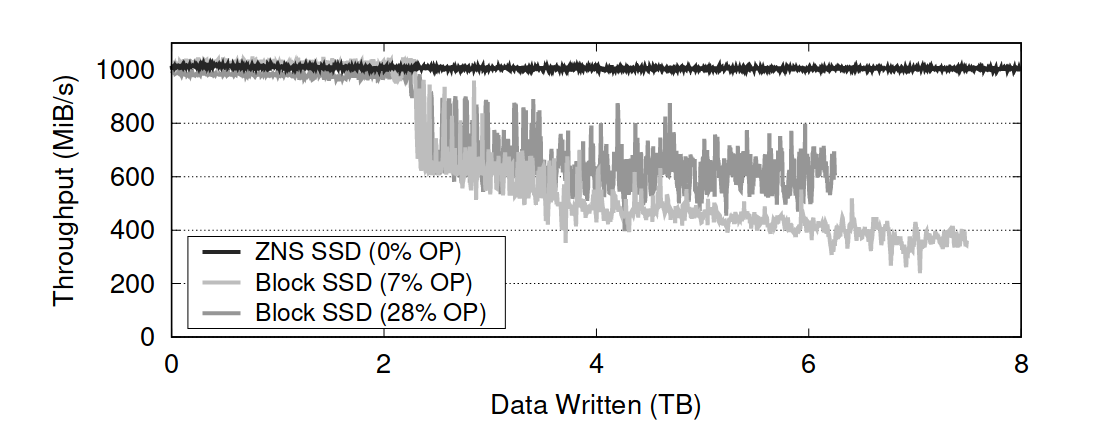
\includegraphics[width=0.8\textwidth]{fig/zns-write}
    \caption{ZNS 多线程完全覆盖写入负载下吞吐量表现}
    \label{zns-write}
\end{figure}

ZenFS 是一种特殊的“文件系统”。与其说是一种文件系统,不如说是一种全新的软硬件协同的系统中的一部分。它通过尽量将原本不可知的 FTL 映射和垃圾回收的过程暴露给上层,使得上层可以更好地利用 SSD 的特性。ZenFS 通过将文件分成多个区域并利用写入生命周期提示来共同定位具有相似生命周期的数据,与传统的块设备相比,系统写入放大大大降低了。ZenFS 确保文件系统或磁盘上没有后台垃圾收集,从而提高吞吐量、尾部延迟和磁盘耐久性方面的性能。

硬件方面,ZenFS 基于 Zoned Storage SSD 和 ZNS(Zoned Namespace SSD)。

ZNS 是 NVMe 最新标准的一部分,它是专用于特殊 SSD 的通用接口,能够将更多的信息暴露到主机上,利用主机的应用场景信息来优化 SSD 的性能。而 Zoned Storage SSD 就是专门为 ZNS 而设计的 SSD,它将 SSD 的内部划分为多个区域,每个区域都有自己的写入指针,不支持随机写入而是只支持从当前写指针写入,从而尽可能地避免了底层主控上的逻辑映射和垃圾回收。普通 SSD 的主控掌握了逻辑地址到物理地址的映射,并且在主机不可控的情况下执行垃圾回收(尽管有 Trim 命令的支持\cite{liang_itrim_2021}),而 Zoned Storage SSD 的垃圾回收机制是由主机来控制的,这样就可以最大程度上地减小写入放大和读写波动,并且能够完全消除硬件预留的空间,从而提高了 SSD 的性能利用率。Zones 的地址空间和写逻辑如图 \ref{zns} 所示。

\begin{figure}[htbp]
    \centering
    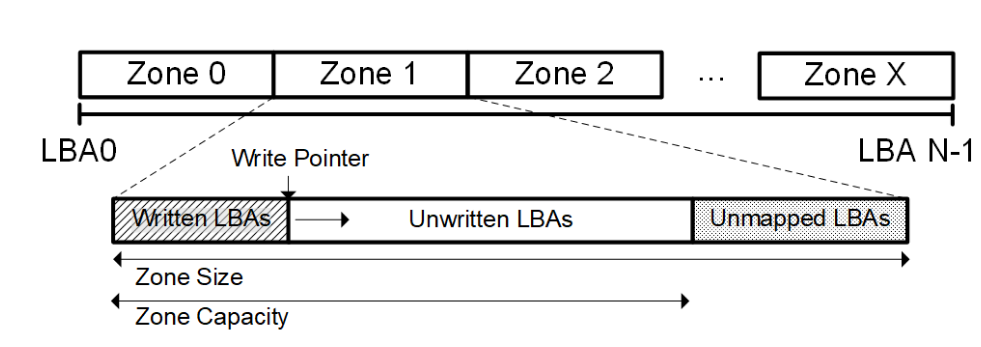
\includegraphics[width=0.8\textwidth]{fig/zns}
    \caption{单个 Zone 内的写逻辑}
    \label{zns}
\end{figure}

硬件方面的尝试其实不止 ZNS 一种。在利用硬件进行 SSD 存储优化的赛道上,有过许多新奇的软硬件技术。Intel 的傲腾就是其中之一,它利用全新的 3D XPoint 相变存储介质,将 SSD 的读写性能提升到了一个新的高度。但是傲腾的缺点也很明显,那就是成本高昂,而且只有 Intel 自家的 CPU 才能够完全发挥傲腾的性能。而 ZNS 和 Zoned Storage SSD 的优势在于,它们是 NVMe 的标准,任何厂商都可以按照标准来生产。而且 ZNS 和 Zoned Storage SSD 的实际生产成本并不高,硬件上主控的计算压力减少了,也释放了更多原来的预留空间,所以大量生产后成本会比现在的 SSD 还要低,因此在可以遇见的未来,ZNS SSD 还会更加普及。

除了傲腾,还有 Open-Channel SSD(OCSSD)\cite{lu_mitigating_2019}。它的主要优化点在于,它将 SSD 的主控和垃圾回收的功能都放到了主机上,而 SSD 只负责读写数据。这样做的好处是,主机可以根据自己的应用场景来优化 SSD 的性能,而且 SSD 的成本也会降低。但是这样做的缺点也很明显,那就是主机的计算压力会变大,而且主机的应用场景也会受到限制。它与 Zoned Storage SSD 的区别主要在于,OCSSD 是将 FTL 放置在主机端,从而减小 SSD 上主控的 DRAM 成本等,而 Zoned Storage SSD 则干脆基本放弃了细粒度的 FTL,只在非常大的 Zone 粒度上做了大块逻辑映射和磨损均衡,从而进一步地让 SSD 服务于计算和存储本身。

\label{zone-type}

在硬件实现上,Zoned Storage SSD 可以设置 Zone 的类型。Zone 可以分为两类:Seq Zone 和 Conv Zone。Seq Zone 正如之前介绍的一样,可以随机读取,但是只能从指定的写指针位置写入数据。而 Conv Zone 则基本可以看作是普通的 SSD,主控仍然会维护这部分地址的 FTL ,所以这部分 Zones 可以像传统 SSD 一般随机读写。这样分类 Zones,更多地是为了兼容现有的应用场景,因为现有的应用场景中,随机读写的需求还是非常多的。而 Seq Zone 则是为了更好地适应新的应用场景,因为新的应用场景中,随机读写的需求并不多,而且 Seq Zone 的性能也更好。

软件方面,ZenFS 则是利用 RocksDB 的文件系统接口将文件放置到原始分区块设备上的区域中。

RocksDB 是 Facebook 开源的一个 KV 存储引擎,它是 LevelDB 的一个分支,主要用于存储 Facebook 的消息系统的元数据。RocksDB 的特点是,它是一个基于 LSM-Tree 的存储引擎,它的读写性能都非常高,而且它的写入放大也非常低。RocksDB 的写入放大主要是通过将写入的数据放到内存中的 MemTable 中,然后再将 MemTable 中的数据写入到磁盘中的 SSTable 中来实现的。RocksDB 的读写性能和写入放大都非常优秀,所以它在 Facebook 的消息系统中得到了广泛的应用。

RocksDB 的 LST-Tree 有多个层次,每个层次都有自己的 SSTable。在 RocksDB 中,每个 SSTable 都是一个文件,而每个 SSTable 中的数据都是有序的。在 RocksDB 中,每个 SSTable 都有一个大小的限制,当 SSTable 的大小达到限制时,就会将达到大小的 SSTable 进行 Compact 操作。LSM-Tree 的操作逻辑(图 \ref{lsm-tree} ),让这种数据结构在磁盘上的表现为一种类似于日志的结构,这样结构的数据库在磁盘上的随机写性能非常高,而且写入放大也非常低。

\begin{figure}[htbp]
    \centering
    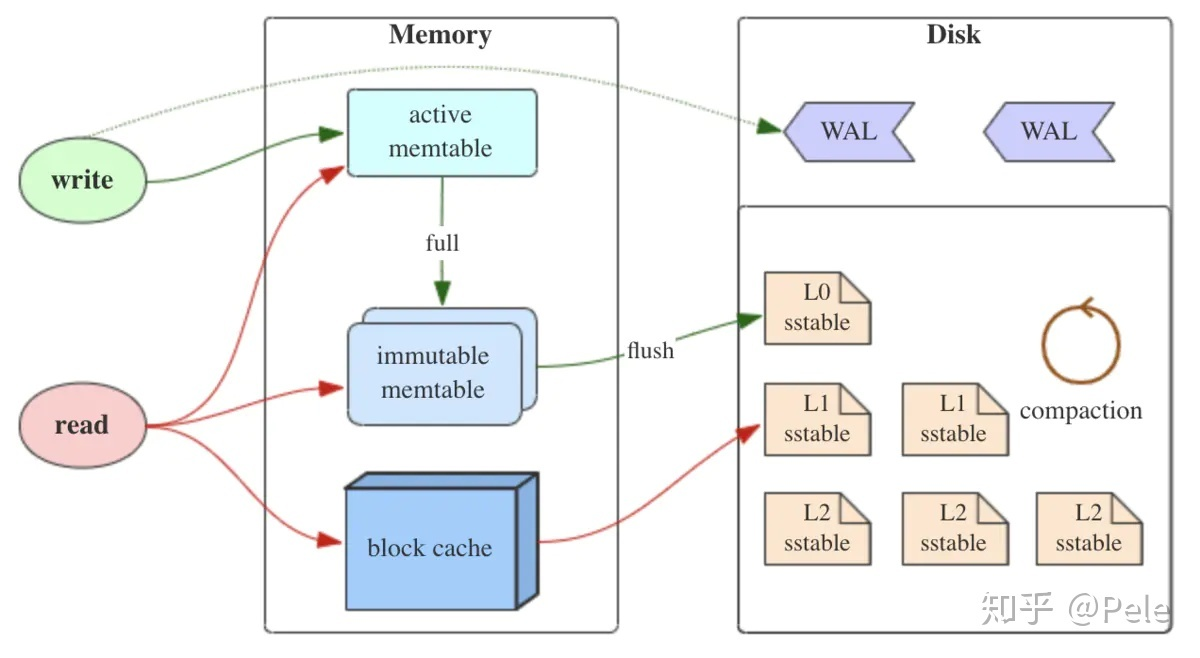
\includegraphics[width=0.8\textwidth]{fig/lsm-tree}
    \caption{LSM-Tree 的操作逻辑}
    \label{lsm-tree}
\end{figure}

在 ZenFS 中,每个上述提到的 SSTable 就是一个 \verb|.sst| 文件。ZenFS 对 SST 文件的管理,也如 SSTable 的完全追加写入如出一辙,即使用 WAL(Write Ahead Log)管理文件的 MetaData 和文件数据,甚至文件的重命名、修改、新增和删除,都是只追加写入的。

\subsubsection{ZenFS 源码分析}

在调研过程中,我们对 ZenFS 的源代码进行了一次完整的分析,总结出我们理解中的 ZenFS 的系统框图(图 \ref{zenfs} )。

\begin{figure}[htbp]
    \centering
    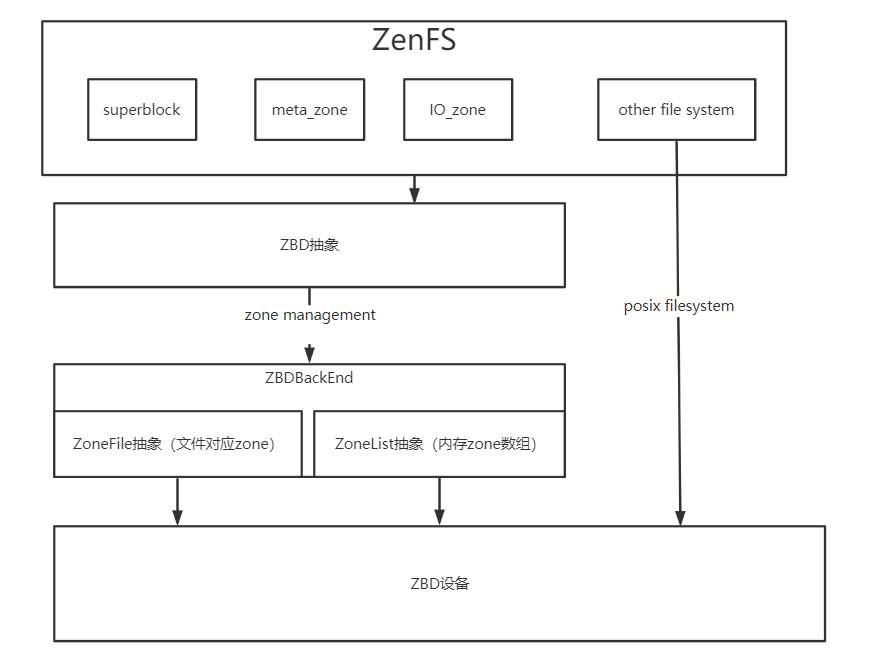
\includegraphics[width=0.8\textwidth]{fig/zenfs}
    \caption{ZenFS 系统框图}
    \label{zenfs}
\end{figure}

\textbf{Zone}

\begin{lstlisting}
  class Zone {
    ZonedBlockDevice *zbd_;
    ZonedBlockDeviceBackend *zbd_be_;
    std::atomic_bool busy_;
    
    uint64_t start_;//起始物理地址
    uint64_t capacity_; /* remaining capacity */
    uint64_t max_capacity_;
    uint64_t wp_;
    Env::WriteLifeTimeHint lifetime_;
    std::atomic<uint64_t> used_capacity_;
  }  
\end{lstlisting}

这里的 Zone 对应的就是设备上的 Zone,不过在 ZenFS 所管理的 Zones 中,只支持 Seq Zone,所以这里的 Zone 也只会是 Seq Zone。

一个Zone需要有所属块设备,起始地址和写指针,生命周期和空间相关的维护。
Zone中的方法有重置Zone,判断是否为空或者是否写满,往写指针后面添加数据等等。

\textbf{ZoneList}

\begin{lstlisting}
  class ZoneList {
    private:
     void *data_;
     unsigned int zone_count_;
   }   
\end{lstlisting}

由于一个 Zoned Storage SSD 上的 Zone 一般比较大,Zone 的数量并不多,所以 ZenFS 要求数据后端要能够快速地提供一个指向 Zones 信息列表的指针,然后通过这个指针就可以快速地求取 Zones 的信息,例如某个 Zone 的起始地址、容量、写指针、是否下线、是否显式打开等。

\textbf{ZonedBlockDeviceBackend}

ZonedBlockDeviceBackend是用来和底层设备交互需要经过的接口,这个接口将底层的ZoneList全部抽象成内存中连续的ZoneList并进行操作。

在 \verb|zbdlib_zenfs.h| 以及 \verb|zbdlib_zenfs.cc| 实现接口以方便上层对底层zbd的访问。

在\verb|zonefs_zenfs.h|以及\verb|zonefs_zenfs.cc|的实现是将上层对zbd的访问通过posix的读写文件方式给包装起来,从而能够访问到被 ZoneFS 包装过后的实际的 Zone。

\begin{lstlisting}
  class ZonedBlockDeviceBackend {
    public:
     uint32_t block_sz_ = 0;
     uint64_t zone_sz_ = 0;
     uint32_t nr_zones_ = 0;
   }   
\end{lstlisting}

backend有两种类型分别是:

\begin{lstlisting}
  enum class BackendType {
    kBlockDev,
    kZoneFS,
  };
\end{lstlisting}

当然,在我们实现了 RAID 之后,这里添加了 backend 类型 kRAID,用来表示这个 backend 是一个 被 RAID 后的数据后端。

\textbf{ZonedBlockDevice}

\begin{lstlisting}
  class ZonedBlockDevice {
    private:
     std::unique_ptr<ZonedBlockDeviceBackend> zbd_be_;
     std::vector<Zone *> io_zones;//用于io的zone
     std::vector<Zone *> meta_zones;//用于保存元信息的zone
     time_t start_time_;
     std::shared_ptr<Logger> logger_;
     uint32_t finish_threshold_ = 0;
     std::atomic<uint64_t> bytes_written_{0};
     std::atomic<uint64_t> gc_bytes_written_{0};// 垃圾回收转移的字节数目
   
     std::atomic<long> active_io_zones_;//分配io_zone时需要用锁
     std::atomic<long> open_io_zones_;
     /* Protects zone_resuorces_  condition variable, used
        for notifying changes in open_io_zones_ */
     std::mutex zone_resources_mtx_;
     std::condition_variable zone_resources_;
     std::mutex zone_deferred_status_mutex_;
     IOStatus zone_deferred_status_;
   
     std::condition_variable migrate_resource_;
     std::mutex migrate_zone_mtx_;
     std::atomic<bool> migrating_{false};
   
     unsigned int max_nr_active_io_zones_;
     unsigned int max_nr_open_io_zones_;
   
     std::shared_ptr<ZenFSMetrics> metrics_;//todo
   }   
\end{lstlisting}

\textbf {Open函数}

用来打开一个ZonedBlockDevice,流程如下:

\begin{itemize}
  \item 首先获取最大活跃io\_zones数目和最大可打开io\_zones,这里保留了几个zone用于metadata存储,一个额外的Zone用于extent migration,即Extent合并时使用的辅助空间。
  \item 从backend中获取已有zones分配3个meta\_zones。将剩余的非离线状态的可获得的zone放入io\_zones中。遍历的过程可统计当前活跃zone的数目。
\end{itemize}

处于离线状态的块,也就是offline,指的是这些块已经在硬件层面检测到错误,不可用了,需要被替换掉。

\textbf {Get*Space函数}:顾名思义,用来获取诸如已经使用空间,空闲空间以及可回收空间大小

\textbf {Log*函数}:用来输出日志,获取zone的整体使用情况,每个zone单个使用情况以及垃圾空间占比等。

\textbf {分配zone区域方法}

ZonedBlockDevice重要的功能应该是操作zone,其分配释放相关操作:

\begin{itemize}
\item ApplyFinishThreshold将剩余空间小于预设的块给finish掉,finish操作指的是把一个zone的写指针移动到zone末尾,剩余容量减为0。
\item FinishCheapestIOZone将一个最小剩余空间的zone给finish。
\item GetBestOpenZoneMatch将一个当前的文件生命周期和每一个io\_zone进行生命周期对比,分配一个生命周期大于当前文件的生命周期且最接近的zone。
\item AllocateEmptyZone,顾名思义是分配一块空的zone。
\item ReleaseMigrateZone,顾名思义是释放migrate\_zone (todo migrate zone是用来干嘛的)。
\item TakeMigrateZone,选择一块最优zone当作migrate\_zone。
\item AllocateIOZone,在保持max\_active\_io\_zones的数量的前提下分配一块zone。
\item Read,从偏移offset处读n个byte吧应该是,这里边用了ZonedDeviceBackend提供的Read接口。
\end{itemize}

而ZonedBlockDevice的读写数据,则基本直接调用ZonedBlockDeviceBackend的相关接口,即交给下一层处理。

\textbf{Snapshot}

ZenFS 的 Snapshot 功能,有多种存储结构的 Snapshot,其记录下某一个确定时间的各个结构的基本信息,从而实现 WAL 结构下的数据一致性保持和快照恢复功能。

几种 Snapshot 的存储结构如下:

\begin{lstlisting}
  // ZBD设备快照记录设备的空闲空间(free_space)
  // 已使用空间(used_space)和可回收空间(reclaimable_space)。
  class ZBDSnapshot {
    public:
     uint64_t free_space;//空闲空间
     uint64_t used_space;//已使用空间
     uint64_t reclaimable_space;//可回收空间
   }

   // Zone快照记录了Zone区域的开始地址(start),写指针(wp),以及容量相关信息。
   class ZoneSnapshot {
    public:
     uint64_t start;//Zone开始地址
     uint64_t wp;//写指针
   
     uint64_t capacity;//容量
     uint64_t used_capacity;//已用容量
     uint64_t max_capacity;//最大容量
   }
   class ZoneExtentSnapshot {
    public:
     uint64_t start;//todo
     uint64_t length;//Extent长度
     uint64_t zone_start;//todo
     std::string filename;//Extent所属文件名
   }
   // 论文中提到过一个文件拥有多个extent,extent不会跨Zone存储
   // 在这些数据结构中可以看出。
   class ZoneFileSnapshot {
    public:
     uint64_t file_id;//顾名思义 file的id
     std::string filename;//文件名
     std::vector<ZoneExtentSnapshot> extents;//文件的extents快照集合
   }
   // 这里的快照便是之前所有快照的组合,记录了整个 ZenFS 设备的重要状态。
   class ZenFSSnapshot {
    public:
     ZBDSnapshot zbd_;
     std::vector<ZoneSnapshot> zones_;
     std::vector<ZoneFileSnapshot> zone_files_;
     std::vector<ZoneExtentSnapshot> extents_;
   };
   
\end{lstlisting}

\textbf{ZoneExtent}

ZoneFs的文件内容是由多个extent组成的,每个extent都放在一个zone里面,extent不能跨zone存储。

\begin{lstlisting}
  class ZoneExtent {
    public:
     uint64_t start_;// 物理起始地址
     uint64_t length_;// extent的长度
     Zone* zone_;// 所属zone指针
   
     explicit ZoneExtent(uint64_t start, uint64_t length, Zone* zone);
     Status DecodeFrom(Slice* input);
     void EncodeTo(std::string* output);
     void EncodeJson(std::ostream& json_stream);
   };   
\end{lstlisting}

\textbf{ZoneFile}

\begin{lstlisting}
  class ZoneFile {
    private:
     const uint64_t NO_EXTENT = 0xffffffffffffffff;
   
     ZonedBlockDevice* zbd_;
   
     std::vector<ZoneExtent*> extents_;
     std::vector<std::string> linkfiles_;
   
     Zone* active_zone_;
     uint64_t extent_start_ = NO_EXTENT;
     uint64_t extent_filepos_ = 0;
   
     Env::WriteLifeTimeHint lifetime_;
     IOType io_type_; /* Only used when writing */
     uint64_t file_size_;
     uint64_t file_id_;
   
     uint32_t nr_synced_extents_ = 0;
     bool open_for_wr_ = false;
     std::mutex open_for_wr_mtx_;
   
     time_t m_time_;
     bool is_sparse_ = false;
     bool is_deleted_ = false;
   
     MetadataWriter* metadata_writer_ = NULL;
   
     std::mutex writer_mtx_;// zonefs的读写锁
     std::atomic<int> readers_{0};
   
    public:
     static const int SPARSE_HEADER_SIZE = 8;
    }   
\end{lstlisting}

ZoneFile是ZenFS中的文件抽象,其记录了文件的元数据信息,包括文件名和路径、时间、文件id、文件大小、文件类型、文件的extents等。

zonefile在操作时只会操作一个active\_zone,同时文件记录了生命周期,读写锁等等。

其中实现的方法有稀疏文件append,所谓稀疏文件就是除了在zone中保存了有效数据信息之外还保存了有效数据的长度信息,如图 \ref{sparse-zone} 所示。

\begin{figure}[htbp]
  \centering
  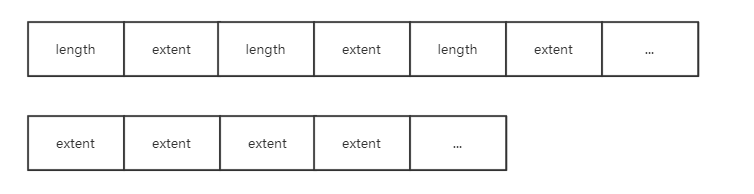
\includegraphics[width=0.8\textwidth]{fig/sparse_zone}
  \caption{ZoneFile 稀疏文件}
  \label{sparse-zone}
\end{figure}

sparse方式的zone中会将长度记录计入,而普通的zone只会一直append文件中的extent。sparse文件能够更加灵活地管理文件的空间,但是会比非sparse文件多一个长度字段信息。

除此之外,zonefs还有实现了RocksDB的FSWritableFile接口以支持顺序写的方法,实现了FSSequentialFile接口以实现顺序读,FSRandomAccessFile接口以实现随机读。

\textbf{SuperBlock}

\begin{lstlisting}
  class Superblock {
    uint32_t magic_ = 0;
    char uuid_[37] = {0};
    uint32_t sequence_ = 0;
    uint32_t superblock_version_ = 0;
    uint32_t flags_ = 0;
    uint32_t block_size_ = 0; /* in bytes */
    uint32_t zone_size_ = 0;  /* in blocks */
    uint32_t nr_zones_ = 0;
    char aux_fs_path_[256] = {0};
    uint32_t finish_treshold_ = 0;
    char zenfs_version_[64]{0};
    char reserved_[123] = {0};
   }  
\end{lstlisting}

ZenFS 的 SuperBlock 超级块相比其他文件系统的超级块要简单很多,其主要记录了一些基本信息,包括魔数、文件系统的版本、block的大小、zone的大小、zone的数量、辅助文件系统路径,之后大部分的信息都是保留字段。

ZenFS 的靠近实际硬件的设计使得它更加简洁高效,但是它的预留修改空间也留足了,为我们今后的修改优化提供了便利。我们全盘 RAID 的实现就是利用了它的超级块的预留空间。

\textbf{ZenMetaLog}

\begin{lstlisting}
  class ZenMetaLog {
    uint64_t read_pos_;
    Zone* zone_;
    ZonedBlockDevice* zbd_;
    size_t bs_;
  }  
\end{lstlisting}

ZenMetaLog 是 ZenFS 的元数据日志格式,是 ZenFS 非常重要的数据存储结构。

zenmetalog加入的record是如图\ref{meta_form}形式,首先存储的是由长度和数据形成的冗余码,然后是数据长度,再是实际的数据。

\begin{figure}[htbp]
  \centering
  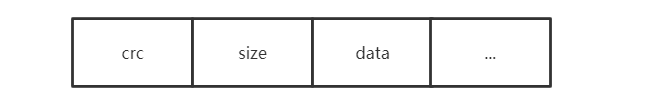
\includegraphics[width=0.8\textwidth]{fig/meta_form}
  \caption{ZenMetaLog Record}
  \label{meta_form}
\end{figure}

每一次roll的操作都会重新开一个zone来记录metadata信息,时机是当这个zone写满了todo,而一个新的metazone的内容首先会加入下面内容,此时记录的是文件系统的瞬时状态也即snapshot,当然这些snapshot是用record的形式加入的(图\ref{roll_metazone_init})。

\begin{figure}[htbp]
  \centering
  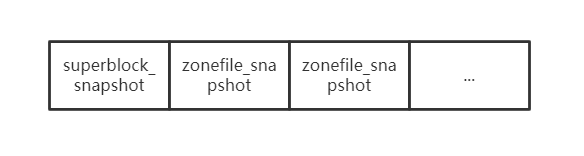
\includegraphics[width=0.8\textwidth]{fig/roll_metazone_init}
  \caption{ZenMetaLog Roll}
  \label{roll_metazone_init}
\end{figure}

在update,replace或是delete文件时,都会按照如图\ref{manipulate_form}格式包装成record加入metalog。

\begin{figure}[htbp]
  \centering
  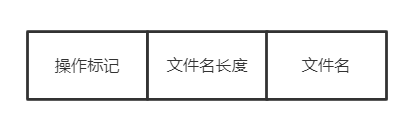
\includegraphics[width=0.8\textwidth]{fig/manipulate_form}
  \caption{ZenMetaLog 格式}
  \label{manipulate_form}
\end{figure}

\textbf{ZenFS}

\begin{lstlisting}
  class ZenFS : public FileSystemWrapper {
    ZonedBlockDevice* zbd_;
    std::map<std::string, std::shared_ptr<ZoneFile>> files_;// ZoneFile
    std::mutex files_mtx_;
    std::shared_ptr<Logger> logger_;
    std::atomic<uint64_t> next_file_id_;
  
    Zone* cur_meta_zone_ = nullptr;
    std::unique_ptr<ZenMetaLog> meta_log_;// 元信息
    std::mutex metadata_sync_mtx_;
    std::unique_ptr<Superblock> superblock_;// 超级块
  
    std::shared_ptr<Logger> GetLogger() { return logger_; }
  
    std::unique_ptr<std::thread> gc_worker_ = nullptr;// 垃圾回收
    bool run_gc_worker_ = false;
  }  
\end{lstlisting}

\textbf{GC\_WORKER垃圾回收}

当全局zone里边的free空间小于一定比例之后,gc\_worker便开始了垃圾回收工作,核心思想便是:

收集需要垃圾回收的zone,即zone的剩余空间满足一定的条件就进行回收,之后将zone中对应的extent移动到与当前zonefile生命周期相匹配的zone,这个zone是顺序写的,这个移动extent的操作叫做migrate操作。

ZenFS 内判断当前zone是否需要回收的条件还是比较简单的,是一个简单的容量判断。当文件系统 GC 时,找到超过容量的 Zone,再找到一个使用较少的 Zone,将超过容量的 Zone 中的数据迁移到使用较少的 Zone 中,就完成了一次 GC。这里ZenFS 简单的实现为我们之后的优化提供了便利。

\textbf{MOUNT逻辑}:

\begin{itemize}
  \item 读入所有metazone并且读出superblock,选择seq序号最大的superblock的meta作为恢复zone。
  \item 若是readonly的,则从磁盘同步一次数据。
  \item 若是可写的,并且用一个新的metazone记录当前文件系统的瞬时状态(superblock以及各个zonefile的编码)。同时要将系统的未用zone重置一下。最后开启垃圾回收线程。
\end{itemize}

\textbf{MKFS逻辑}:

\begin{itemize}
  \item 选择一个metazone作为log记录的zone。
  \item 写入superblock和各个zonfile编码到metazone中。
\end{itemize}

以上基本基于源码结构对 ZenFS 做了一个简单的分析。有了以上的理解分析,我们就可以开始对 ZenFS 进行修改优化了。
    \section{系统设计}

AquaFS 是一个模块化的文件系统,以下是 AquaFS 的整体架构图:

\subsection{AquaFS 整体架构}

\begin{figure}[H]
    \centering
    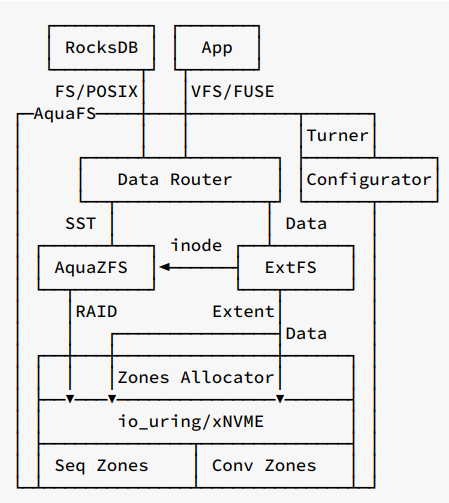
\includegraphics[width=0.8\textwidth]{fig/aquafs-frame}
    \caption{AquaFS 整体架构图}
    \label{aquafs-frame}
\end{figure}

架构图 \ref{aquafs-frame} 中的模块简略说明如下:

\begin{enumerate}
    \item App:文件系统请求负载
    \item RocksDB:数据库请求
    \item Data Router:FileSystem 请求路由器,需要判断当前请求是否适合 WAL 优化
    \item Turner:动态调整运行过程中的参数
    \item Configurator:静态调整文件系统参数,建立文件系统时给出建议参数
    \item AquaZFS:经过修改和优化的 ZenFS,支持 RAID 等功能
    \item ExtFS:有 inode 系统的运行于 Seq/Conv Zones 上的通用文件系统
        \begin{enumerate}
            \item 对普通请求,直接使用 Conv Zones
            \item 对 AquaZFS 的新文件,提供 inode 索引等读写优化
            \item 对较大的冷数据文件,分配到 Seq Zones
            \item 将一些可以异地更新的数据以 AquaFS::Extent 形式写入 AquaZFS
        \end{enumerate}
    \item Zones Allocator:为 AquaZFS、ExtFS 提供 Zone 分配服务
    \item Zones:
        \begin{enumerate}
            \item Seq Zones:只能顺序写的 Zones
            \item Conv Zones:可以随机写的 Zones
        \end{enumerate}
    \item AquaFS:整体文件系统
\end{enumerate}

\subsection{模块设计细节}

\subsubsection*{RocksDB 使用 AquaFS}

RocksDB 使用 AquaFS,可以走两种数据通路:FileSystem 和 POSIX 接口。

\textbf{RocksDB 使用 FileSystem 接口使用 AquaFS}

将 AquaFS 编译为 RocksDB 插件,Data Router 使用 FileSystem 接口。

Data Router 主要转发 SST 请求到 AquaZFS,其他请求转发到 ExtFS,并对特殊情况做二者的负载均衡。

\textbf{RocksDB 使用 POSIX 接口使用 AquaFS}

AquaFS 的 Data Router 通过 Kernel Module 或 FUSE 提供 POSIX 访问接口,并智能判断数据负载位置。

\subsubsection*{App 使用 AquaFS}

由于假定 App 并未实现 FileSystem 接口,所以 App 数据可以通过 Kernel Module / FUSE 方式经过 Data Router 到下层。

\subsubsection*{调参模块}

AquaFS 中调参模块主要有两个部分:Configurator、Turner。

Configurator 在文件系统创建前评估当前系统更适合的固定参数,并结合需求给出合适的参数选择和预估的性能区间。

Turner 在文件系统使用过程中保持运行,根据系统当前状态动态调整可改变的参数,以获得更加灵活良好的整体表现。

\textbf{可调参数}

\begin{enumerate}
    \item 固定参数
    \begin{enumerate}
        \item 块大小
        \item 固定 RAID 参数
        \item 数据后端类型
    \end{enumerate}
    \item GC
    \begin{enumerate}
        \item GC 容量阈值
        \item GC 间隔时间
    \end{enumerate}
    \item 动态 RAID
    \begin{enumerate}
        \item 分配时间(GC)
        \item 分配参数(0/1/5...)
    \end{enumerate}
    \item 文件请求分类
    \begin{enumerate}
        \item 分类为 SST、普通数据
        \item 分类冷热文件/数据
    \end{enumerate}
    \item IO 加速方式:io\_uring/xNVME
\end{enumerate}

\subsubsection*{AquaZFS 和 ExtFS}

ExtFS 是主要运行于 Conv Zones 上的针对 ZNS 优化的文件系统。主要特性:

\begin{enumerate}
    \item 必须原地更新的数据放在 Conv Zones 内,如 Superblock 等(?)
    \item 适合异地更新的数据通过 AquaZFS 保存在 Seq Zones 内,如 MetaData(?)
    \item 如果智能检测到 AquaZFS 内部分数据不适合 Seq Zones 存储,则转发到 ExtFS 内处理
    \item 用冗余的 inode 等为 AquaZFS 提供索引,可以动态降低其内存消耗
\end{enumerate}

AquaZFS 是基于 ZenFS 的优化修改,支持以上特性,在保存高性能的同时提升文件系统的灵活性。

\subsubsection*{RAID}

在 AquaZFS 从写盘前到实际写盘之间,存在一层 RAID 逻辑。

在原版 ZenFS 的实现中并没有实现 RAID 的逻辑,其只能保证存储的“记录”的数据正确性,而无法保证“文件”的数据正确性,
也不能在遇到磁盘故障的时候自动处理修复数据。

AquaZFS 在 ZenFS 的基础上实现了 RAID 逻辑,可以在磁盘故障时自动修复数据,且能够根据配置自动使用不同的 RAID 策略。

除了保证数据的正确性,AquaZFS 还可以根据不同的 RAID 策略提供不同的性能。
当前实现的 RAID0 可以以 N 倍加速单线程数据的读写,RAID1 在提供 N 倍读性能的同时,还可以用简单的冗余策略保证数据的安全性。

AquaZFS 的 RAID 有两种基本模式:全盘模式和智能动态分区模式。

在全盘模式下,AquaZFS 会以 SSD 设备为单位应用同一种 RAID 策略,其策略配置写入超级块中,
可以快速将已经在使用的 AquaZFS 转换为 全盘 RAID 格式,并使用超级块在 Meta Zones 中的追加写入逻辑保证配置的正确性。

在智能动态分区模式下,AquaZFS 以 Zones 为单位配置 RAID 策略,可以在不同的 Zones 中使用不同的 RAID 策略。
RAID 策略信息以记录形式写入 Meta Zones 中,并使用 WAL 配合 Snapshot 保证数据的正确性。

在实现的过程中,我们为其他的 RAID 逻辑做了预留,能够快速地实现其他 RAID 逻辑。

\begin{enumerate}
    \item 可灵活配置为:静态固定参数 RAID、智能动态分区 RAID
    \item 可以在用户态驱动 NVME,或者内核态使用 liburing 进行 IO 加速,充分利用多盘优势提升性能
    \item 利用 Turner 提供的建议,在 AquaZFS 垃圾回收时或合并 Extent 时调整 RAID 逻辑,使文件系统在安全性、性能上有更好的权衡点
\end{enumerate}

\subsubsection*{Zones Allocator}

为 AquaZFS 和 ExtFS 提供统一的 Zones 分配服务。

\begin{enumerate}
    \item 让整盘空间得到更加充分的利用,减少由于分开两种子系统造成的空间碎片
    \item 根据历史数据,测算不同 Zones 的寿命和速度,来控制 Zones 的分配逻辑,延长磁盘寿命,提高磁盘吞吐
\end{enumerate}

\subsubsection*{IO 加速}

在 AquaFS 向上提供 FileSystem 接口时,由于负载程序对 FileSystem 接口做了适配,所以可以让负载程序和整个 AquaFS 都跑在用户态。

当 AquaFS 整个运行在用户态,可以使用 xNVME 用户态 NVME 协议驱动,降低内核态用户态切换的性能损失,同时也可用 io\_uring 加速。

若 AquaFS 使用 POSIX 接口,可以使用 VFS 或者 FUSE 接口,此时也可以用 xNVME 或者 io\_uring 进行 IO 加速。

\subsubsection*{智能化}

这个架构的「智能」体现在哪?

\begin{enumerate}
    \item 相比与 ZenFS,灵活性更强
    \begin{enumerate}
        \item 适配没有针对优化的工作负载,智能识别适合 WAL 的数据,用更合适的方式处理
        \item 可调整的静态、动态参数更多
        \item 提供 RAID 功能,并可以动态分配
    \end{enumerate}
    \item 数据安全性更强:RAID 功能
    \item 智能分配请求
    \begin{enumerate}
        \item 在 Data Router 层合理分配 SST、普通数据请求
        \item 在当前请求不适合 AquaZFS 的时候将 ExtFS 作为后备
        \item 进行读写请求分离
    \end{enumerate}
\end{enumerate}


    \section{系统实现}

针对以上设计,我们实现了 AquaFS 文件系统。
AquaFS 文件系统的实现基于 ZenFS,我们在 ZenFS 的基础上进行了修改和优化,使其支持 RAID 等功能。

\subsection{AquaFS 文件系统的 RAID 实现}

RAID 是指独立冗余磁盘阵列(Redundant Array of Independent Disks),它是一种数据存储技术,通过将多个硬盘组合起来,实现数据的备份、容错和性能优化。

当我们确定 RAID 方案的时候,首先需要解决的问题是:如何将 ZNS 中的 Zones 组织成 RAID 单位。在传统的 RAID 实现中,RAID 单位是磁盘,而在 ZNS 中,RAID 单位可以是磁盘,也可以是 Zone。我们既可以将 ZNS 中的 Zones 组织成 RAID 单位,也可以将 ZNS 中的磁盘组织成 RAID 单位。我们将 ZNS 中的 Zones 组织成 RAID 单位的方式称为分区 RAID,将 ZNS 中的磁盘组织成 RAID 单位的方式称为全盘 RAID。

那么我们是否能将所有的 Zones 都组织成 RAID 单位呢?答案是否定的。在 Zoned Storage SSD 中,Zone 分为了两种:Seq Zone 和 Conv Zone。更详细的说明在 \ref{zone-type}。这两种 Zones 由于其读写方式的区别,是不能混为一谈的。如果将 Seq Zone 和 Conv Zone 混用,则浪费了主控上专门对 Conv Zones 配置的 DRAM Cache,也会降低 Seq Zone 的读写性能。所以,我们不能将所有的 Zones 都组织成 RAID 单位,而是需要将 Seq Zone 和 Conv Zone 分开组织成 RAID 单位。

除了 Zone 类型的问题,基于 Zone 的 RAID 对磁盘之间的参数也提出了要求。在相同参数的 Zoned Storage SSD 中,不同设备上的 Zone 由于 Zone 大小、块大小等是相同的,可以很方便地组合为 RAID 单位。但是,如果不同设备上的 Zone 参数不同,那么就不能直接组合为 RAID 单位。所以,我们首先实现的是将相同参数的 Zone 组合为 RAID 单位,对不同参数的 Zone 组合为 RAID 单位的实现将在复赛阶段进行探索,例如进行参数转换、分区兼容等尝试。

除此之外,在 ZNS 上实现 RAID 还需要解决 Seq Zones 上的 RAID 算法问题。RAID 0 与 RAID 1 的逻辑相对简单,而 RAID 5、RAID 6 等则需要在 Seq Zone 上实现更复杂的 RAID 算法。这些算法需要文件系统进一步实现各个 Zones 的读写缓存、原子同步写入等功能。我们尝试了 RAID 5 的算法,但是运行效果暂时不理想。在 ZNS 上实现 RAID 5、RAID 6 等算法的难度较大,我们决定在复赛阶段进行探索。

当前 AquaFS 的 RAID 实现主要分为两种:全盘 RAID 和分区 RAID。这两种 RAID 实现的区别在于,全盘 RAID 的 RAID 单位是磁盘,而分区 RAID 的 RAID 单位是 Zone。

\subsubsection{全盘 RAID 的实现}

在传统的 RAID 实现中,基本都是以磁盘为单位进行数据 RAID 逻辑。以磁盘为单位的 RAID 能够充分运用各个磁盘的数据吞吐,并基于 Linux 的块设备等抽象层提供软件上的 RAID 功能。我们也首先实现了全盘 RAID 的功能,能够将多个 ZNS 配置为 RAID 0、RAID 1 模式。

由于 ZenFS 是一个没有一般 POSIX 接口的文件系统,其仅向上服务于 RocksDB,所以我们并不能简单地使用 Linux 上常用的磁盘软件 RAID 来实现 ZNS 的 RAID 功能。更何况,ZNS 并不是 Linux 兼容的块设备,内核中并没有对 ZNS 的 RAID 支持。经过调研和评估,我们认为在 Linux Kernel 内实现对 ZNS 的 RAID 支持并不现实。于是,我们需要在 ZenFS 的基础上实现 RAID 功能。

ZenFS 的数据读写将会经过以下几个层次:

\begin{enumerate}
  \item RocksDB 的 SSTable
  \item RocksDB 的 MemTable
  \item RocksDB 的 WAL
  \item RocksDB 的 FileSystem
  \item ZenFS 的 ZoneFile
  \item ZenFS 的 ZoneExtent
  \item ZenFS 的 Record
  \item ZenFS 的 ZonedBlockDeviceBackend
  \item libzbd 的 ZbdlibBackend
  \item Linux Kernel 相关系统调用
\end{enumerate}

其中,RocksDB 的 SSTable、MemTable、WAL、FileSystem 都是 RocksDB 的内部实现,ZenFS 的 ZoneFile、ZoneExtent、Record、ZonedBlockDeviceBackend 都是 ZenFS 的内部实现,libzbd 的 ZbdlibBackend 是 ZenFS 内对 libzbd 的接口适配,Linux Kernel 相关系统调用是 libzbd 作为用户态程序调用 Linux Kernel 内的设备驱动程序的接口,最终还是会通过 Linux 的系统调用来实现数据的传输。

ZenFS 和 RocksDB 还支持了另一种数据读写方式,通过 ZoneFS 将 ZNS 中的 Zones 以文件映射到文件系统中,然后通过文件系统的接口来读写数据。这种方式的数据读写流程如下:

\begin{enumerate}
  \item RocksDB 的 SSTable
  \item RocksDB 的 MemTable
  \item RocksDB 的 WAL
  \item RocksDB 的 FileSystem
  \item ZenFS 的 ZoneFile
  \item ZenFS 的 ZoneExtent
  \item ZenFS 的 Record
  \item ZenFS 的 ZonedBlockDeviceBackend
  \item ZoneFS 的 ZoneFSBackend
  \item Linux Kernel VFS 接口
\end{enumerate}

虽然这种方式通过 ZoneFS 将 ZNS 中的 Zones 以文件映射到文件系统中,但是 ZoneFS 并不是一个通用的文件系统,它仅仅是一个将 ZNS 中的 Zones 以文件的形式映射到文件系统中的文件系统。ZoneFS 并不支持文件的创建、删除、重命名等操作,文件的读写操作也支持不完全,而且还会引入更多的存储 IO 栈,所以我们并没有选择通过 ZoneFS 来实现 ZNS 的 RAID 功能。

我们选择在 ZenFS 的 ZonedBlockDeviceBackend 层实现 ZNS 的 RAID 功能。ZonedBlockDeviceBackend 层是 ZenFS 中管理数据后端的层,它是 ZenFS 与 libzbd 或 ZoneFS 之间的接口层,负责将 ZenFS 的数据读写请求转换为 libzbd 或 ZoneFS 的数据读写请求。

我们通过继承 ZonedBlockDeviceBackend 来实现 ZenFS 内的数据 RAID 功能。ZonedBlockDeviceBackend 的继承类图如图 \ref{raid-layers} 所示。

\begin{figure}[htbp]
  \centering
  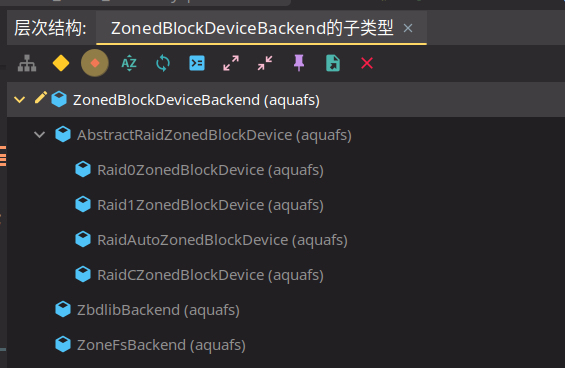
\includegraphics[width=0.85\textwidth]{fig/raid-layers}
  \caption{ ZonedBlockDeviceBackend 继承类图 }
  \label{raid-layers}
\end{figure}

AbstractRaidZonedBlockDevice 下的 Raid0ZonedBlockDevice、Raid1ZonedBlockDevice 和 RaidCZonedBlockDevice 即为全盘 RAID 的实现。其中,Raid0ZonedBlockDevice 实现了 RAID 0 的功能,Raid1ZonedBlockDevice 实现了 RAID 1 的功能,RaidCZonedBlockDevice 实现了 RAID C 的功能。

RAID C 是我们自定义的一种简单 RAID 格式,它通过 Zones 的合并来实现简单的数据拼合逻辑,即将多个 Zone 合并为一个 Zone,然后将数据写入到合并后的 Zone 中。RAID C 的实现如图 \ref{raid-c} 所示。

\begin{figure}[htbp]
  \centering
  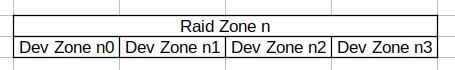
\includegraphics[width=0.85\textwidth]{fig/raid-c}
  \caption{ 全盘 RAID 的数据排布 }
  \label{raid-c}
\end{figure}

此时多个($m$个)设备上实际存在的 Zones 合并为一个大的逻辑 Raid Zone,数据将会按顺序依次写入 Dev Zone $n_{i}$($0 \le i < m$)。此 RAID C 模式存在的意义是,形成一个简单的 Zone 合并逻辑,便于后续开发应用。其中,Dev Zone $n_i$ 分别为来自第 $i$ 个设备的第 $n$ 个 Zone。

RAID 0 和 RAID 1 的实现与传统的 RAID 0 和 RAID 1 的实现类似,RAID 0 将数据分散写入多个设备中,RAID 1 将数据写入多个设备中的一个。RAID 0 和 RAID 1 的实现中的数据排布与 RAID C (图 \ref{raid-c})基本一致。

传统块设备上 RAID 0 的工作原理如下:

\begin{enumerate}
  \item 数据被分割成固定大小的块。
  \item 这些块按照一定的规则,如轮流或按块交替,分配到不同的物理磁盘驱动器上。
  \item 每个磁盘驱动器只存储一部分数据,因此所有磁盘驱动器都可以同时读写数据,从而提高了读写速度。
  \item 当需要读取数据时,RAID控制器会从所有驱动器中读取数据块,然后将它们组合成完整的数据块,并将其发送给请求数据的主机。
\end{enumerate}

RAID 0 在写入时,将会将数据分散写入多个设备中。类似于传统块设备的 Block Size,ZNS 也是有最小写入单位的,也是 Block Size。RAID 0 在读写时,可以将读写请求分割为不同的 Block Size 的读写请求,然后对这些请求重新合并排序,再调用底层的读写接口。

当前我们的实现中,RAID 0 的实现基本与传统 RAID 0 一致。区分的点有以下几个:

\begin{enumerate}
  \item 数据需要以 Zone 为单位做组织,而不是以设备为单位。即与传统 RAID 0 的最后向上层应用提供一个抽象磁盘设备不同,我们需要向上层应用提供多个抽象的 Zones。
  \item 数据被分为不同的 Block Size 的块,分得尽量小。
  \item 当需要读写数据时,RAID 0 会将读请求分割为不同的 Block Size 的读写请求,然后对这些请求重新合并排序,再调用底层的读接口。
  \item 采用了 Direct IO 加速方案,即绕过 Page Cache,直接读写设备。
  \item 采用了 io\_uring 加速方案,即使用 io\_uring 作为异步 IO 框架,提高 IO 吞吐量。
\end{enumerate}

以 RAID 0 读为例,其未经 IO 优化的读流程如下所示:

\begin{lstlisting}
int Raid0ZonedBlockDevice::Read(char *buf, int size, uint64_t pos,
                                bool direct) {
#ifndef AQUAFS_RAID_URING
  // split read range as blocks
  int sz_read = 0;
  int r;
  while (size > 0) {
    auto req_size =
        std::min(size, static_cast<int>(GetBlockSize() - pos % GetBlockSize()));
    r = devices_[get_idx_dev(pos)]->Read(buf, req_size, req_pos(pos), direct);
    if (r > 0) {
      size -= r;
      sz_read += r;
      buf += r;
      pos += r;
    } else {
      return r;
    }
  }
  return sz_read;
#else
  // ...
#endif
}
\end{lstlisting}

代码逻辑主要为,每次请求最多读取一个 Block Size 的数据,然后将读取的数据拼接到 buf 中,直到读取完毕。其中需要多次重复计算数据分块的设备位置和块位置,于是这里使用了 get\_idx\_dev 和 req\_pos 函数来快速计算设备位置和块位置。这些函数被实现在 AbstractRaidZonedBlockDevice 层,以便其子类可以快速调用其逻辑。

在上述代码中,我们将读请求分割为不同的 Block Size 的读请求,然后调用底层的读写接口。这样做的好处是,可以将读请求分散到多个设备中,从而提高读性能。不过,上述代码中其实并没有体现 RAID 0 的多设备读优化,还是单线程读取。我们在后文中实现了基于 uring 的多设备并行读优化。

除了读写逻辑,RAID 还需要抽象出 Zones 的统一管理。上层软件使用了 RAID 向上提供的抽象 RAID Zones,那么对这些抽象 RAID Zones 的各种 Zone 操作也应当起到作用。例如,对 RAID 0/1 Zone 的重置操作应当扩散到这个 RAID Zone 对应的所有 Dev Zones;对求一个 RAID Zone 的逻辑写指针值,也应该按照 RAID 逻辑计算逻辑 RAID Zone 内的容量,然后计算已用容量,最后计算出逻辑写指针值。对 Zones 的 Close、Finish 等操作的逻辑类似。

当使用全盘 RAID 1 的时候,还有个可以优化的点,即当组成 RAID 的设备的参数相同时,由于这些设备的 Zone 大小相同,因此可以将这些设备的 Zone 一一对应起来,从而利用写指针的对应关系,不需要对请求进行切分,减轻了一些计算上的开销。

\subsubsection{智能分区 RAID 的实现}

分区 RAID 的实现与全盘 RAID 的实现类似,但是我们在逻辑 Raid Zone 和实际设备 Zone 之间加上了一层基于 Zones 的映射。这些映射是通过 ZenFS 的 Record 写入 MetaZones 内的,将在每次文件系统加载的时候逐步读取加载映射逻辑。

加上这一层映射之后,分区 RAID 的数据排布逻辑可能如图 \ref{raid-a} 所示。

\begin{figure}[htbp]
  \centering
  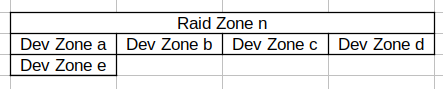
\includegraphics[width=0.85\textwidth]{fig/raid-a}
  \caption{ 分区 RAID 的数据排布 }
  \label{raid-a}
\end{figure}

Zone Raid $n$ 为向上层暴露出的可读写数据 Zone 区域,而其中可以存在多种不同的 RAID 逻辑或映射类型。

在示例图 \ref{raid-a} 中,Dev Zone $x$ 表示来自不同或相同设备的设备上物理存在的 Zone。
如果这个 Raid Zone 被配置为 RAID 1,则 Dev Zone $a$ 和 Dev Zone $e$ 将同时以 RAID 1 数据冗余方式为 Raid Zone $n$ 的前四分之一数据提供服务,其他 Dev Zones 由于没有映射,将回退到 RAID C 逻辑提供数据存储服务。若这个 Raid Zone 被配置为 RAID 0,则 Dev Zone $a$ 和 Dev Zone $e$ 将同时以 RAID 0 数据分散方式为 Raid Zone $n$ 的前四分之一数据提供服务,其他 Dev Zones 由于没有映射,将回退到 RAID C 逻辑提供数据存储服务。

实际代码实现上,除了上述映射逻辑处理,还有许多细节需要考虑。

\textbf{物理块逻辑设备均分问题}:在抽象 RAID Zone 里的 Zones 中,这些块可以来自不同的设备,也可以来自同一个设备。但是为了最大化利用 ZNS 的带宽,我们需要尽量将数据分散写入不同的设备中。

\textbf{跨 Zones 读写问题}:由于我们添加的映射逻辑,使得我们的数据排布不再是连续的,而是以 Zones 为单位分散的。这就导致了我们的读写请求可能会跨越多个 Zone。这就需要我们在读写时,需要将读写请求分割为不同的 Block Size 的读写请求,然后可能对这些请求重新合并排序,再调用底层的读写接口。

在读或写代码中,通过数据段分割并递归调用自身的方式实现跨 Zones 读写的请求分割:

\begin{lstlisting}
  if (static_cast<decltype(zone_sz_)>(size) > zone_sz_) {
    // may cross raid zone, split read range as zones
    int sz_read = 0;
    int r;
    while (size > 0) {
      auto req_size =
          std::min(size, static_cast<int>(zone_sz_ - pos % zone_sz_));
      r = Read(buf, req_size, pos, direct);
      if (r > 0) {
        buf += r;
        pos += r;
        sz_read += r;
        size -= r;
      } else {
        return r;
      }
    }
    // flush_zone_info();
    return sz_read;
  } else {
    // ...
\end{lstlisting}

\textbf{数据后端问题}:由于我们是基于 ZonedBlockDeviceBackend 来实现的,而 ZonedBlockDeviceBackend 有多种子类,可以是 libzbd、ZoneFS 甚至是原来实现的全盘 RAID。
为了进一步简化 IO 调用栈,我们在实现分区 RAID 时,假定数据后端都是 libzbd 提供的数据读写。这在之后可以进一步优化,以支持更多的数据后端,提升 RAID 逻辑的灵活性,如添加 ZoneFS 支持、添加 SPDK 等 Kernel bypass 方案支持等。

\textbf{对 ZenFS 的兼容性问题}:ZenFS 在加载的过程中,会对固定的 MetaZones 进行扫描,通过 Magic Number 查找到 Meta Zones 中的可用的超级块,并选择最新的超级块进行文件系统初始化。为了兼容 ZenFS 的 Meta Data 管理逻辑,我们不能改变 MetaZones 的排布,也不能改变超级块的存储逻辑。因此,我们在实现分区 RAID 时,需要保证 MetaZones 的排布不变,超级块的存储逻辑不变,以及超级块的存储位置不变。所以,我们在实现分区 RAID 时,将 MetaZones 的排布和超级块的存储位置都固定在了第一个设备上,进行映射的连续逻辑预分配,这样就可以保证 ZenFS 的兼容性,使得 ZenFS 在加载分区 RAID 时,可以正常加载。

在创建或读取文件系统时的预分配映射:

\begin{lstlisting}
  // create temporal device map: AQUAFS_META_ZONES in the first device is used
  // as meta zones, and marked as RAID_NONE; others are marked as RAID_C
  for (idx_t idx = 0; idx < AQUAFS_META_ZONES; idx++) {
    for (size_t i = 0; i < nr_dev(); i++)
      allocator.addMapping(idx * nr_dev() + i, 0, idx * nr_dev() + i);
    allocator.setMappingMode(idx, RaidMode::RAID_NONE);
  }
\end{lstlisting}

为了管理分区之间的映射关系,我们通过组合的方式实现了一个分区分配器 ZoneRaidAllocator。其可以管理分区的映射关系,以及分区的 RAID 逻辑。其主要接口如下:

\begin{lstlisting}
  Status addMapping(idx_t logical_raid_zone_sub_idx, idx_t physical_device_idx,
                    idx_t physical_zone_idx);
  void setMappingMode(idx_t logical_raid_zone_idx, RaidModeItem mode);
  void setMappingMode(idx_t logical_raid_zone_idx, RaidMode mode);

  int getFreeDeviceZone(idx_t device);
  int getFreeZoneDevice(idx_t device_zone);
  Status createMapping(idx_t logical_raid_zone_idx);
  Status createMappingTwice(idx_t logical_raid_zone_idx);
  Status createOneMappingAt(idx_t logical_raid_zone_sub_idx, idx_t device,
                            idx_t &zone);
  void setOffline(idx_t device, idx_t zone);
\end{lstlisting}

其可以提供映射关系的查询、增加、删除、修改等功能,以及提供 Raid Zone 所分配的 RAID 逻辑的查询、增加、删除、修改等功能。

同时,它还提供了 setOffline 功能,可以在发现设备故障时,将故障设备的所有分区设置为 Offline 状态,以便后续的故障处理。

\subsubsection{分区 RAID 故障处理}

在分区 RAID 故障处理方面,我们实现了基于分区 RAID 的故障处理方案。其主要思路是,当发现设备故障时,将故障设备的所有分区设置为 Offline 状态,然后将所有的分区重新映射到其他设备上,以保证数据的可用性。

由于在调研中我们发现,Nand Flash 向上提供的数据一般含有 ECC 校验和纠错,且 ZenFS 中的 Record 也有 CRC 校验和,所以我们认为在数据传输过程中,较少比特数据的完整性是可以保证的。所以,我们在实现分区 RAID 故障处理时,仅考虑大块数据的完整性恢复,而不考虑小块数据的完整性。

\begin{lstlisting}
  // 在数据操作函数中
  if (r < 0) {
    auto status = ScanAndHandleOffline();
    if (status.ok()) {
      // retry this read
      return Read(buf, size, pos, direct);
    } else {
      Error(logger_, "failed to restore data: %s", status.getState());
      return r;
    }
  }
\end{lstlisting}

ScanAndHandleOffline 函数将扫描当前所有盘的数据状态,如果发现有盘处于 Offline 状态,则将所有的分区重新映射到其他设备上,并根据 RAID 逻辑进行数据恢复。

当前由于仅实现了 RAID 0 和 RAID 1 的数据逻辑,所以暂时仅支持 RAID 1 分区的数据恢复。当发现 RAID 1 分区的数据不一致时,将重新选择一个 Dev Zone,将数据恢复到新的 Dev Zone 上。

当前的故障处理逻辑还相对比较简单,在复赛中实现更多 RAID 逻辑后,将进一步改进此部分的故障处理逻辑,如增加 RAID 5 的故障处理逻辑、增加故障恢复的并发度等。

\subsection{AquaFS 的 IO 加速实现}

在上文中,我们已经介绍了 AquaFS 的 RAID 方案,但是由于是比较初级的版本,很多代码并没有进行并行优化,仍然是单线程的。所以,我们在实现 IO 加速方面,主要是对 RAID 下的 IO 操作进行并行优化。

在我们实现之前,ZenFS 的 IO 优化主要是从 RocksDB 中继承而来。RocksDB 中可以使用 Direct IO 来读写文件,以避免数据在用户态和内核态之间的拷贝。其 Direct IO 优化既可以用于 RocksDB 的 PosixFileSystem 常规文件系统后端,也可以用于 RocksDB 的 ZenFS 文件系统后端。

Direct IO 主要的优化逻辑是,将用户态的数据缓冲区直接映射到内核态的页缓存中,从而避免了数据在用户态和内核态之间的拷贝。通过 Direct IO 打开的设备,从设备中获得的数据将直接写入在用户态的数据缓冲区中,而不是先写入内核态的页缓存中,从而减少了一次数据拷贝。

Direct IO 的使用也非常简单,只需要在打开文件时,将 O\_DIRECT 标志传入即可。但是,由于 Direct IO 的使用需要满足一些条件,如文件的偏移量和长度需要是当前系统内存页大小的整数倍,所以在使用 Direct IO 时,需要对读写对应的内存缓冲区地址和长度进行对齐。具体对齐方式为使用 \verb|posix_memalign| 函数来申请内存,控制参数将申请的内存地址对齐到当前系统内存页大小的整数倍。

\begin{lstlisting}
  ret = posix_memalign((void**)&buffer, sysconf(_SC_PAGESIZE), phys_sz);
\end{lstlisting}

我们发现,在我们的加速方案中,Direct IO 可以与更多的 IO 加速方案并存。如在我们的加速方案中,我们可以使用 io\_uring 来加速 IO 操作,而 io\_uring 也可以与 Direct IO 并存。

在加速方案选择上,我们选择了 io\_uring 方案。当前 Linux 系统上有许多 IO 加速方案,如 AIO、io\_uring、libaio 等,如图 \ref{io-speedup} 所示。

\begin{figure}[htbp]
  \centering
  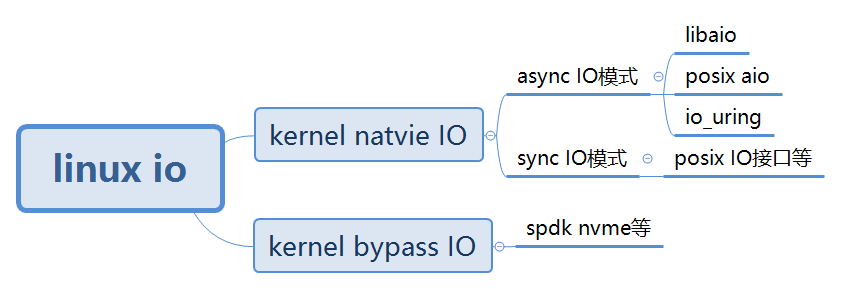
\includegraphics[width=0.7\textwidth]{fig/io-speedup}
  \caption{IO 加速方案}
  \label{io-speedup}
\end{figure}

io\_uring 是 kernel natvie aio 的一种,它是 Linux Kernel 5.1 版本加入一个特性。io\_uring 围绕高效进行设计,其设计了一对共享的 ring buffer 用于应用和内核之间的通信,通过该设计实现了如下的三个好处:

\begin{enumerate}
  \item 避免在提交和完成事件中存在内存拷贝;
  \item 避免了 libaio 中在提交和完成任务的时候系统调用过程;
  \item 该队列采用了无锁的访问模式,通过内存屏障减少了竞争。
\end{enumerate}

io\_uring 的使用也非常简单,只需要提交 SQE 到 ring buffer 中,然后等待 CQE 即可。
由于其简单使用、高效的设计,我们选择了 io\_uring 作为我们的 IO 加速方案。

其实 io\_uring 在 RocksDB 的 PosixFileSystem 文件系统后端中已经有可选的实现,但是它并没有被实现到 ZenFS 后端中,ZenFS 的数据读写还是只能使用 Direct IO 进行优化。于是,我们在 ZenFS 的文件系统后端中实现了 io\_uring 的优化,从而进一步加速了 ZenFS 的 IO 操作。

为了进一步增大 IO 加速的效果,我们还实现了 IO 操作的批处理。在原版 ZenFS 中,IO 操作是以单个系统调用的形式进行的,即每次 IO 操作都是单个请求。但是如果将多个 IO 操作打包成一个批处理请求,可以进一步提高 IO 操作的效率,尤其是单 IO 请求的效率。

为了实现 IO 操作的批处理,我们在 AquaZFS 的文件系统后端中实现了 IO 请求的分割和合并,并将请求全部打包成一个批处理请求,然后一次性提交给 io\_uring,从而实现了 IO 操作的批处理。

除了上述优化处理,我们还使用 C++ 20 的协程特性,进一步增大了代码的并行性。
在调研过程中,我们找到了一个 C++ 实现的 io\_uring 绑定库,其向外提供了协程接口,可以在协程中使用 io\_uring。我们将其移植到了 AquaFS 中,从而实现了在协程中使用 io\_uring。

有关逻辑可以在数据操作相关的函数中找到,如下以读数据函数 Read 为例:

\begin{lstlisting}
  using req_item_t = std::tuple<int, char *, uint64_t, off_t>;
  std::vector<req_item_t> requests;
  std::vector<ZbdlibBackend *> bes(nr_dev());
  for (decltype(nr_dev()) i = 0; i < nr_dev(); i++) {
#ifdef ROCKSDB_USE_RTTI
    bes[i] = dynamic_cast<ZbdlibBackend *>(devices_[i].get());
    assert(bes[i] != nullptr);
#else
    bes[i] = (ZbdlibBackend *)(devices_[i].get());
#endif
  }
  while (size > 0) {
    // ...
    requests.emplace_back(fd, buf, req_size, mapped_pos);
    // ...
  }
\end{lstlisting}

如上所示,我们首先将 IO 请求分割成多个小的 IO 请求,将这些请求收集到 std::vector 中。
由于 ZNS 支持随机读,所以可直接将 IO 请求加入到 std::vector 中,而无需考虑 IO 请求的顺序。

收集到 IO 读请求后,我们将这些请求打包成一个批处理请求,然后一次性提交给 io\_uring,如下所示:

\begin{lstlisting}
  uio::io_service service;
  // ...
  service.run([&]() -> uio::task<> {
    std::vector<uio::task<int>> futures;
    for (auto &&req : requests) {
      uint8_t flags = 0;
      // read do not need order
      // if (req != *req_list.second.cend()) flags |= IOSQE_IO_LINK;
      futures.emplace_back(service.read(std::get<0>(req), std::get<1>(req),
                                        std::get<2>(req), std::get<3>(req),
                                        flags) |
                           uio::panic_on_err("failed to read!", true));
    }
    for (auto &&fut : futures) co_await fut;
  }());
\end{lstlisting}

在作为举例的 Read 函数中,我们首先创建了一个 service 对象,然后使用 run 方法启动协程,在协程中逐个将请求提交到 SQE 中,然后等待所有的 CQE 即可。这里的 flags 参数用于指定 IO 请求的属性,如 IOSQE\_IO\_LINK 表示该 IO 请求是一个批处理请求中的一部分。由于我们的 IO 请求是无序的,所以我们不需要使用 IOSQE\_IO\_LINK。

在写操作相关的函数中,相比于读操作,还需要基于 ZNS 的顺序写特性考虑更多的因素,如下所示:

\begin{lstlisting}
  using req_item_t = std::tuple<char *, uint64_t, off_t>;
  // <dev, zone> -> vec<ordered req>
  std::map<std::pair<int, idx_t>, std::vector<req_item_t>> requests;
\end{lstlisting}

我们首先将 IO 请求按照设备和 Zone 序号进行分组,然后将每个 Zone 内的 IO 请求按照顺序进行排序,最后将这些请求收集到 std::vector 中。而在提交 IO 请求时,我们需要将这些请求按照顺序依次提交。

总之,我们在 AquaFS 中实现了 io\_uring 和 C++20 协程 的优化,从而进一步加速了 AquaFS 的 IO 操作。

\subsection{AquaFS 文件系统的智能调参模块实现}

智能调参模块方面,实现了基于方差的重要参数选择方案和基于高斯过程回归的参数调整方案。

\begin{figure}[htbp]
  \centering
  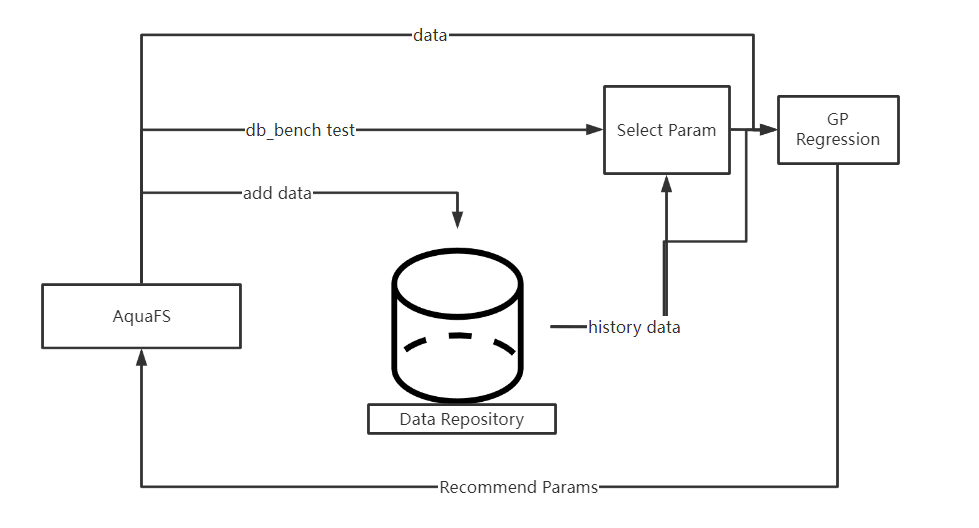
\includegraphics[width=0.7\textwidth]{fig/aquaturnner}
  \caption{AquaTurnner 智能调参模块}
  \label{aquaturnner}
\end{figure}

如图 \ref{aquaturnner} 所示,AquaTurnner 智能调参模块主要由三部分组成,被调对象,本文中是AquaFS,历史数据存储仓库,以及调参事务组成,调参事务又包括选择参数选择模块和高斯过程回归调整参数模块。

首先,AquaFS需要预热地运行,收集到不同参数配置下的目标指标,本文中使用的是吞吐量指标,将对应的参数配置和目标指标值存入数据仓库中。在初次预热之后,后续不须要预热,除非加入了新的参数指标。

考虑到AquaFS作为RocksDB的插件存在,在本文中使用RocksDB的测试脚本db\_bench来测试系统的吞吐量,采用prometheus作为收集数据的工具。在这个测试中,用收集到的目标指标值和配置参数值,配合历史数据仓库中的数据,来进行参数选择和高斯过程回归。参数选择模块根据方差指标选择最重要的几个参数,高斯过程回归用重要的参数和目标指标值进行拟合以及回归。

首先对于最重要的参数,由方差计算的最大值对应的参数得到:

\begin{equation}
  \label{eq:var}
  \begin{aligned}
    Var(S)=\frac{1}{\lvert S\rvert}\sum_{i=1}^{\lvert S\rvert}(y_i-\mu)^2 \\
    PI(P)=Var(S)-\sum_{i=1}^{N}\frac{S_{P=P_i}}{S}Var(S_{p=p_i})
  \end{aligned}
\end{equation}

这里的 $y_i$ 是样本中的目标值,$\mu$ 是样本目标值均值,$PI$ 系数是基于方差来计算的,即固定某一个参数的值,根据参数的值划分集合,在每个集合中求出集合中目标值的对应方差,再用初始方差 $Var(S)$ 减去这个和,这个 $PI$ 系数越大说明原来的这个参数的影响越大,因为在同一个值的情况下,集合内方差的和很小。

其次由 $CPI$ 指标来选择剩余重要参数:

\begin{equation}
  \label{eq:cpi}
  \begin{aligned}
    CPI(Q|P=p) = Var(S_{P=p})-\sum_{j=1}^{m}\frac{S_{Q=Q_{w_j},P=p}}{S_{P=p}}Var(S_{Q=q_i|P=p})\\
    CPI(Q|P=p) = \max_{1\le i\le n}CPI(Q|P=p_i)
  \end{aligned}
\end{equation}

基于方差的重要参数选择算法如算法 \ref{alg:aquaturnner_select} 所示。

\begin{algorithm}[htb]
  \caption{ AquaTuner参数选择算法 }
  \label{alg:aquaturnner_select}
  \begin{algorithmic}[1]
    \Require
      adjust\_param\_num, db\_bench\_data, data in repository
    \Ensure
      important\_params
    \State important\_params = []
    \State Select the most important param by $PI(param)$, add to important\_params;
    \State For $i$ in adjust\_param\_num $–$ $1$:
    \State \qquad Compute $CPI$ for each param that not in important\_params;
    \State \qquad Select the largest $CPI$’s corresonding params to important params; \\
    \Return important\_params
  \end{algorithmic}
\end{algorithm}

对于连续参数,AquaTuner对于参数指标在参数范围内给出合适的推荐参数值,该合适参数值是在拟合的高斯过程模型曲线上,根据在最优配置参数附近做抖动获得,也即尝试最优配置参数点附近的参数值看目标指标是否有所提升,对于离散参数,AquaTunar尝试匹配最优目标指标值对应的配置参数的离散值。

AquaTuner的运行算法流程如算法 \ref{alg:aquaturnner_trunning} 所示。

\begin{algorithm}[htb]
  \caption{ AquaTuner参数调优算法 }
  \label{alg:aquaturnner_trunning}
  \begin{algorithmic}[2]
    \Require
      adjust\_param\_num
    \Ensure
      recommend\_param
    \State data repository <- warm up system and collect data;
    \State start db\_bench;
    \State db\_bench\_data = collect data from db\_bench;
    \State add db\_bench\_data to data repository;
    \State important\_params = Select\_Param(adjust\_param\_num ,db\_bench\_data, data in repository);
    \State GP\_model = GP\_regression(important\_params, eb\_bench\_data, data in repository);
    \State recommend\_param = [];
    \State For param in  history\_best\_params and important params:
    \State \qquad If param is continuous:
    \State \qquad \qquad Try values near the past value, add to recommend\_param;
    \State \qquad Else if param is discrete:
    \State \qquad \qquad Try values in best params,add to recommend\_param;
    \State Target = GP\_model.predict(recommend\_param);
    \State If Target is better:
    \State \qquad \Return recommend\_param;
    \State \Return history\_best\_param;
  \end{algorithmic}
\end{algorithm}

    \section{系统测试}

\subsection{智能分区 RAID 模块和 IO 加速测试}

由于 ZNS 当前仅有西数公司的设备支持,我们原本预计使用西数的 ZNS SSD 进行测试,即 SN530 512GB。但是由于西数的 SSD 申请过程非常复杂,国内外沟通流程也比较慢,现在仍在处理流程中,我们无法在短时间内获得设备,只能使用仿真环境进行测试。

在几个月前,FAST23 上有一篇关于 ZNS 的论文,它类似 SPDK,在用户态实现了 NVME 的协议,也包括了 ZNS 的协议,可以在 Linux 上模拟 ZNS SSD。但是我们在测试过程中发现,它的 ZNS 模拟实现有问题,无法正常使用,我们在 Github 上提了 issue,但是现在项目还在持续更新中,我们测试中遇到的问题只解决了一些,但是又有更多新的问题出现。我们尝试去解决这些问题,但是由于时间有限,我们最终无法在初赛前解决这些问题,只能放弃在初赛中使用这个模拟器。

以下 RAID IO 测试均使用了基于数据的延迟计算仿真,即计算 SSD 的访问延迟和数据传输延迟,其数据存储后端是内存。由于内存的访问延迟远小于 SSD,因此可以忽略内存的访问延迟,只计算 SSD 的访问延迟和数据传输延迟。

测试环境为:Intel(R) Core(TM) i7-12700 CPU,内存 40GB 3200MHz;系统为 Archlinux,Linux 内核版本 6.3.5-arhc1-1。由于 libzbd、ZoneFS、nvmevirt 等都需要比较高的内核版本,于是这里直接一步到位地使用了最新的 Linux Kernel mainline。

\subsubsection{数据完整性测试}

由于 AquaZFS 是作为一个插件运行在 RocksDB 的文件系统层上的,所以可以使用 RocksDB 来验证其数据完整性。我们使用 RocksDB 的 db\_bench 工具进行测试,测试结果如表 \ref{test-data} 所示。

\begin{table}[htbp]
  \centering
  \caption{数据完整性测试}
  \label{test-data}
  \begin{tabular}{cccc}
    \hline
    \textbf{测试项} & \textbf{设备数} & \textbf{测试参数} & \textbf{测试结果} \\
    \hline
    全盘 RAID C & 2 & \verb|--fs_uri=aquafs://raidc:dev:nullb0,dev:nullb1| & 通过 \\
    全盘 RAID 0 & 2 & \verb|--fs_uri=aquafs://raid0:dev:nullb0,dev:nullb1| & 通过 \\
    全盘 RAID 1 & 2 & \verb|--fs_uri=aquafs://raid1:dev:nullb0,dev:nullb1| & 通过 \\
    分区 RAID A & 2 & \verb|--fs_uri=aquafs://raida:dev:nullb0,dev:nullb1| & 通过 \\
    \multirow{2}{*}{分区 RAID A} & \multirow{2}{*}{4} & \verb|--fs_uri=aquafs://raida:dev:nullb0,dev:nullb1,| & \multirow{2}{*}{通过} \\
    & & \verb|dev:nullb2,dev:nullb3| & \\
    \hline
  \end{tabular}
\end{table}

db\_bench 除了表 \ref{test-data} 中的,还需要添加如下参数:

\begin{lstlisting}
./plugin/aquafs/aquafs
  mkfs # 创建文件系统
  # --raids= 此选项用于指定数据后端,这里指定使用 AquaFS 的 RAID 功能
  --aux_path=/tmp/aquafs # 指定 AquaFS 的辅助数据存储路径,如锁文件和日志缓存文件
  --force # 清除原有的文件系统数据

./db_bench 
  # --fs_uri= 此选项用于指定数据后端,可以是文件系统路径,也可以是 AquaFS 的相关配置
  --benchmarks=fillrandom # 指定测试项,使用随机写并校验
  --use_direct_io_for_flush_and_compaction # 使用 Direct IO 加速
  --use_stderr_info_logger # 在标准错误输出日志
\end{lstlisting}

由于输出较多,这里仅展示一部分输出,如图 \ref{check-data1}、\ref{check-data2}、\ref{check-data3} 所示。

\begin{figure}[htbp]
  \centering
  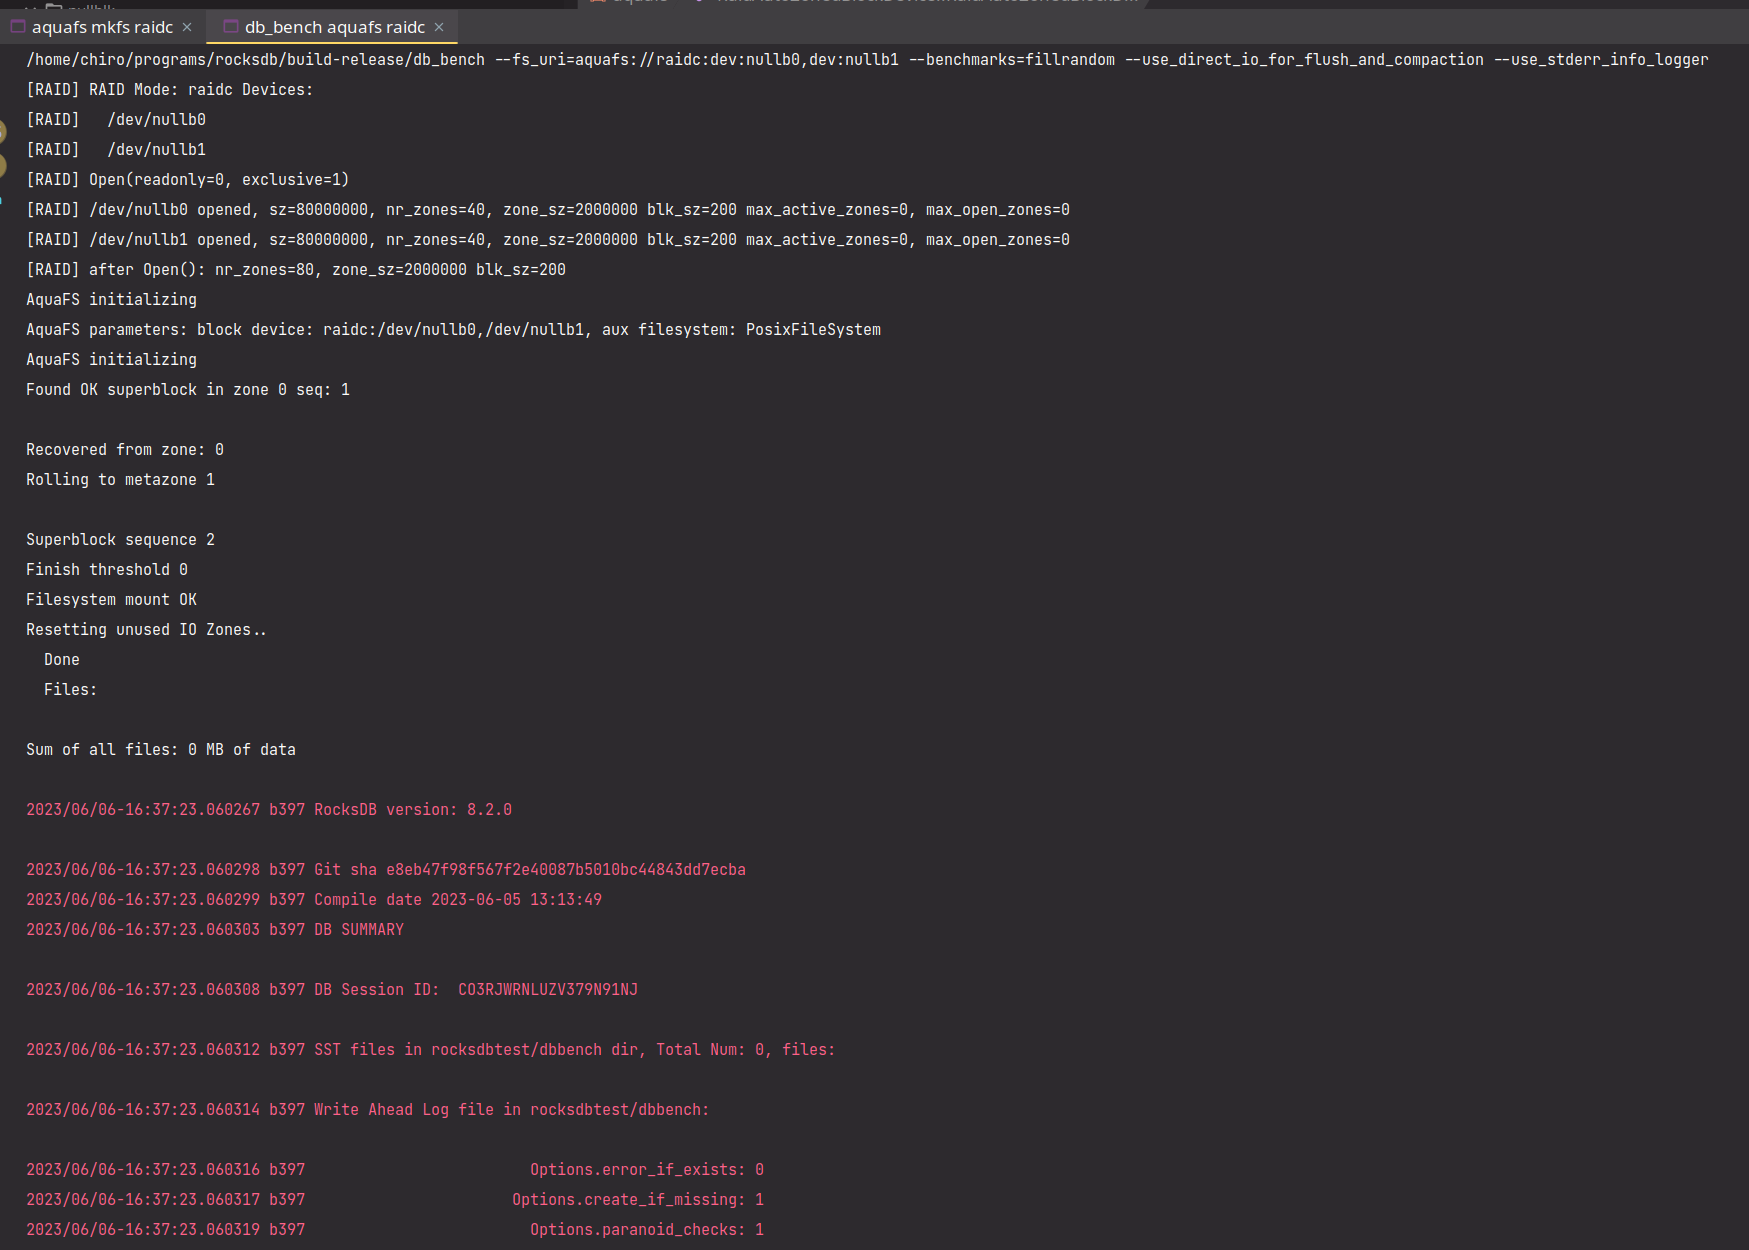
\includegraphics[width=0.85\textwidth]{fig/raid-data-check1.png}
  \caption{ 数据完整性测试1 }
  \label{check-data1}
\end{figure}

\begin{figure}[htbp]
  \centering
  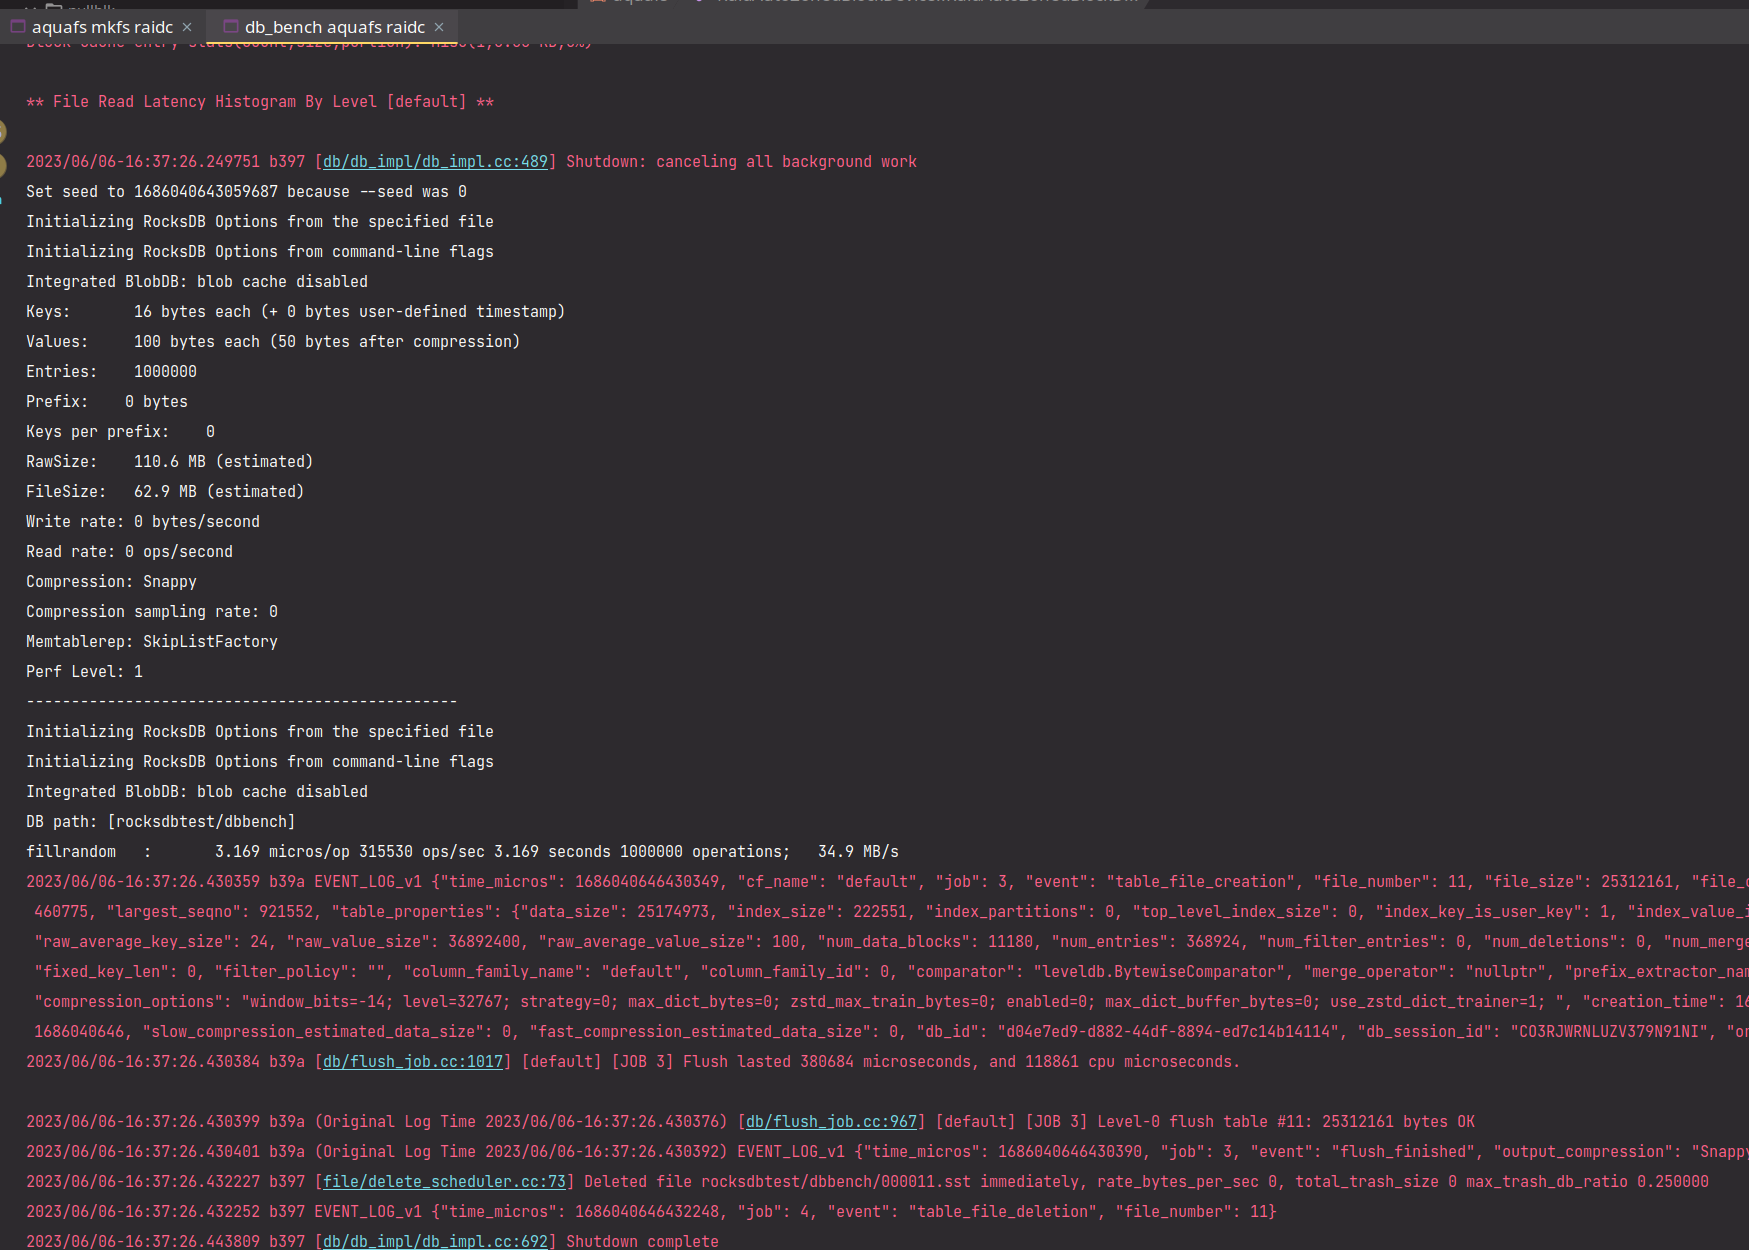
\includegraphics[width=0.85\textwidth]{fig/raid-data-check2.png}
  \caption{ 数据完整性测试2 }
  \label{check-data2}
\end{figure}

\begin{figure}[htbp]
  \centering
  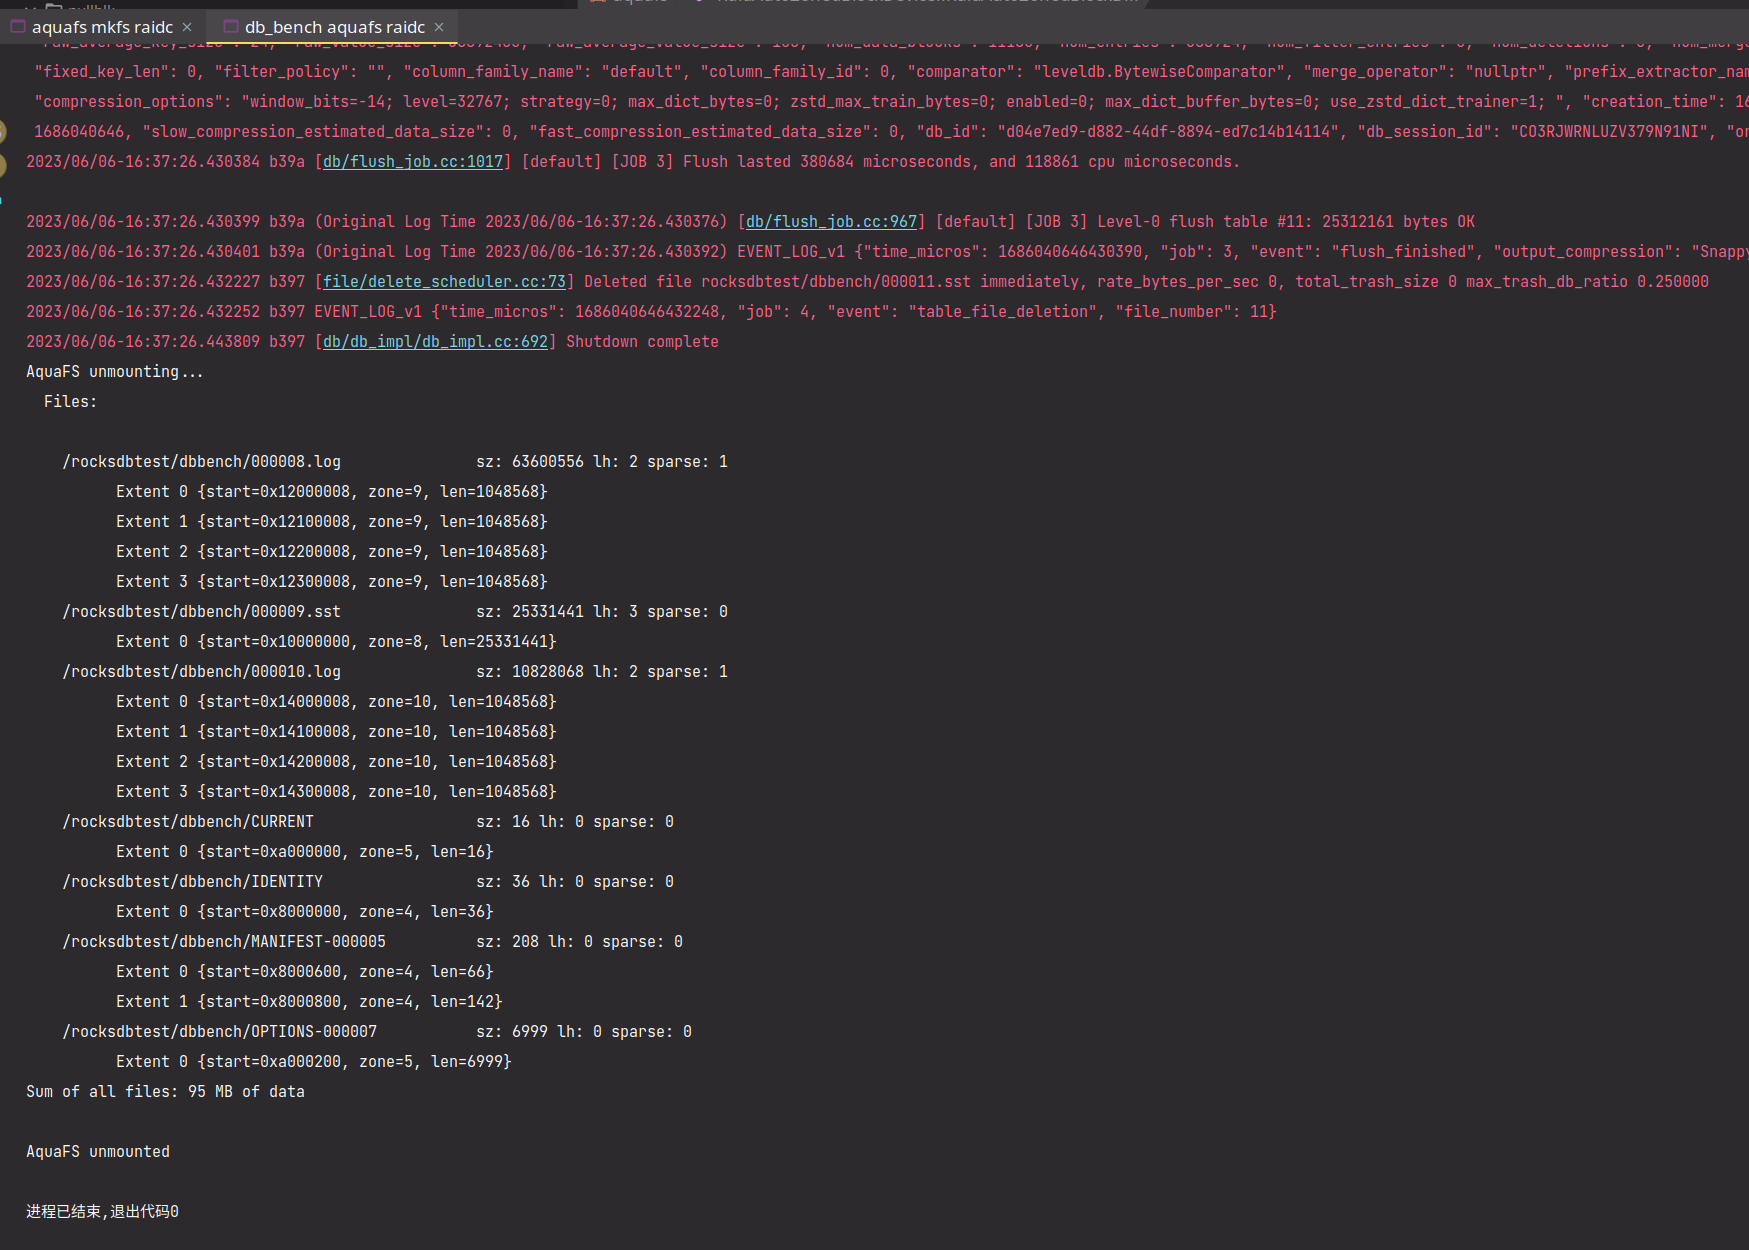
\includegraphics[width=0.85\textwidth]{fig/raid-data-check3.png}
  \caption{ 数据完整性测试3 }
  \label{check-data3}
\end{figure}

\subsubsection{使用 RAID 0 加速文件读写}

由于 ZenFS 并不支持 POSIX 规范的文件系统访问接口,所以无法将其挂载到 Linux 的 VFS 上,因此无法使用 Linux 的文件系统测试工具来测试其性能。这里使用的测试逻辑,与 RocksDB 使用 AquaFS 文件系统插件类似,都是通过写程序调用 AquaFS 的 API 来测试性能。

使用如下逻辑测试文件读写性能,并比较 RAID 0 的性能加速:

\begin{enumerate}
  \item 生成测试参数,包括文件大小、设备数量、RAID逻辑、随机种子等
  \item 创建文件系统,设置RAID逻辑等
  \item 在内存中生成一个指定大小的随机内容文件
  \item 重复进行多次:
  \begin{enumerate}
    \item 通过 \verb|aquafs restore| 将这个文件写入 AquaFS 文件系统
    \item 通过 \verb|aquafs dump| 将文件从 AquaFS 文件系统读出
    \item 通过 \verb|std::hash| 和 \verb|md5sum| 比较读出的文件和原文件是否一致
  \end{enumerate}
  \item 计算平均耗时,得到读写平均时间
\end{enumerate}

对多组数据进行测试,结果输出如图 \ref{raid0-speedup} 所示:

\begin{figure}[htbp]
  \centering
  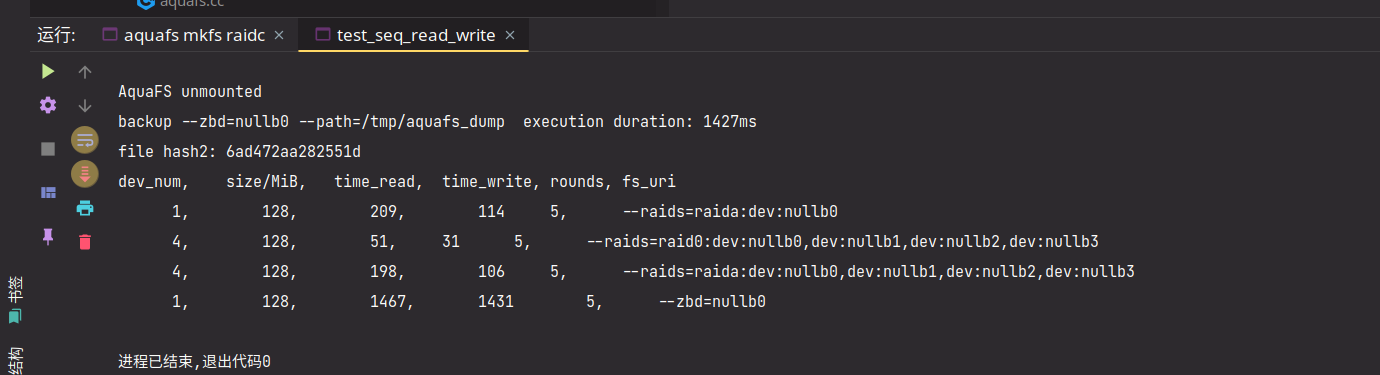
\includegraphics[width=0.85\textwidth]{fig/raid0-speedup.png}
  \caption{ RAID 0 加速测试 }
  \label{raid0-speedup}
\end{figure}

其得到的数据如表 \ref{raid0-speedup-table} 所示:

\begin{table}[htbp]
  \centering
  \caption{RAID 0 加速测试}
  \label{raid0-speedup-table}
  \begin{tabular}{cccccc}
    \hline
    \textbf{设备数量} & \textbf{文件大小(MiB)} & \textbf{平均读时间(ms)} & \textbf{平均写时间(ms)} & \textbf{次数} & \textbf{说明} \\
    \hline
    1 & 128 & 209 & 114 & 5 & 单盘分区 RAID \\
    4 & 128 & 51 & 31 & 5 &  多盘全盘 RAID 0 \\
    4 & 128 & 198 & 106 & 5 &  多盘分区 RAID \\
    1 & 128 & 1467 & 1431 & 5 &  ZenFS 默认 \\
    \hline
  \end{tabular}
\end{table}

可以看到,在单盘分区 RAID 的情况下,读写性能都有至少 N 倍的性能提升,而在多盘全盘 RAID 0 的情况下,读写性能有更大提升。

相比与 ZenFS 的默认读写,单盘分区读写由于使用 io\_uring、协程、重新构造读写请求等方式,性能有成倍的提升。具体提升幅度被能同时读写的 Zone 数量限制;而原版 ZenFS 只能单线程进行数据请求,因此性能较低。

相比与单设备的分区 RAID,多盘分区 RAID 有更大的性能提升。多盘意味着系统并行度更大,因此获得了更高的瞬时吞吐量。

而多盘全盘 RAID 0,由于采用的读写加速方式与分区 RAID 一致,其逻辑更加精简,因此性能更高。

\subsubsection{文件系统数据恢复测试}

测试逻辑:

\begin{enumerate}
  \item 生成随机大文件
  \item 使用 \verb|aquafs restore| 将文件写入 AquaFS 文件系统
  \item 在软件层面触发模拟硬件故障,使得一个 Dev Zone 下线
  \item 使用 \verb|aquafs dump| 将文件从 AquaFS 文件系统读出,观察是否能够正常读出
  \item 校验读出的文件和原文件是否一致
\end{enumerate}

使用 128 MiB 文件大小进行测试,测试过程如图 \ref{test-recovery} 所示。
在测试中,AquaFS 成功地检测到了 Zone 的故障,并且成功地从其他 Zone 中恢复了数据,维护了文件系统的数据完整性。

\begin{figure}[htbp]
  \centering
  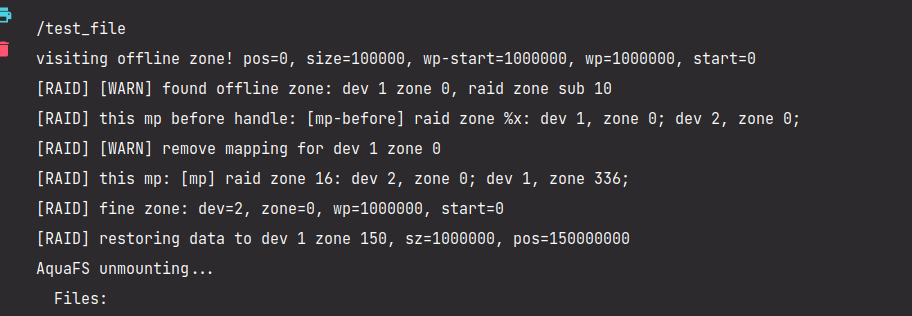
\includegraphics[width=0.85\textwidth]{fig/test-recovery.png}
  \caption{ 数据恢复测试 }
  \label{test-recovery}
\end{figure}

\subsubsection{文件系统性能测试}

由于可以使用内存作为存储后端,我们可以很便利地分析 AquaFS 的性能瓶颈,从而快速优化其性能。

我们使用 Linux \verb|perf| 工具进行性能分析,其中部分分析过程如图 \ref{test-perf} 所示。

\begin{figure}[htbp]
  \centering
  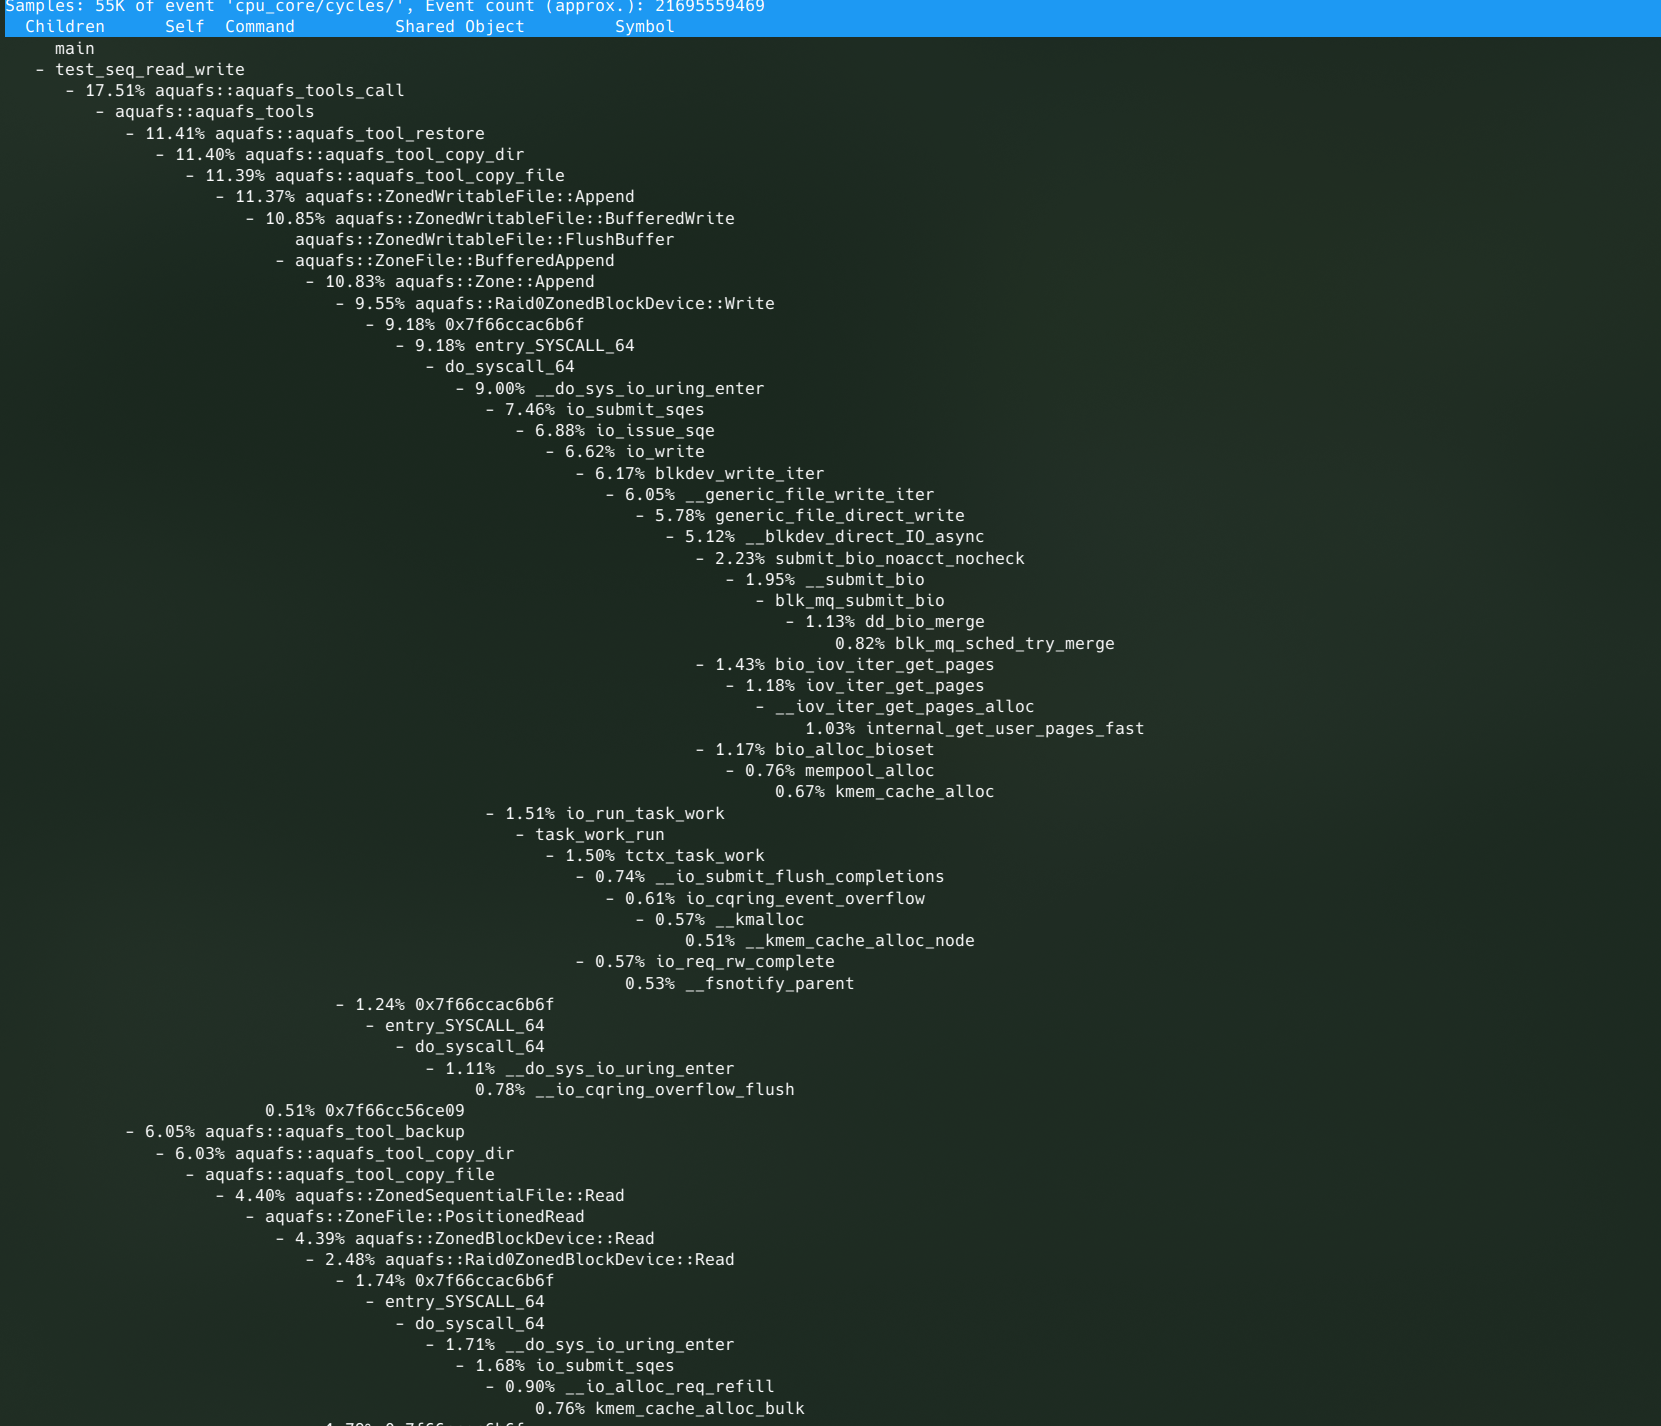
\includegraphics[width=0.85\textwidth]{fig/test-perf.png}
  \caption{ perf 性能分析 }
  \label{test-perf}
\end{figure}

可以看到,AquaFS 的性能瓶颈主要在于:

\begin{enumerate}
  \item \verb|entry_SYSCALL_64|:当前仍然使用内核态的 \verb|open|、\verb|read|、\verb|write| 等系统调用,导致系统频繁地从用户态切换到内核态,导致性能瓶颈。
  \item \verb|io_submit_sqes|:正在使用 io\_uring 的软件层面实现,可能使用方法还有可以优化的地方,造成 io\_uring 中一部分数据的锁争用。
\end{enumerate}

\subsection{AquaTurnner 智能调参模块测试}

首先进行warm\_up得到一组参数和目标指标值的csv文件如图 \ref{test-turnner1} 所示,现在由于只调整AquaFS参数,参数空间较小,主要包括垃圾回收的gc相关参数,块大小以及zone的大小参数等,后续考虑在融合文件系统后加入inode相关参数。

\begin{figure}[htbp]
  \centering
  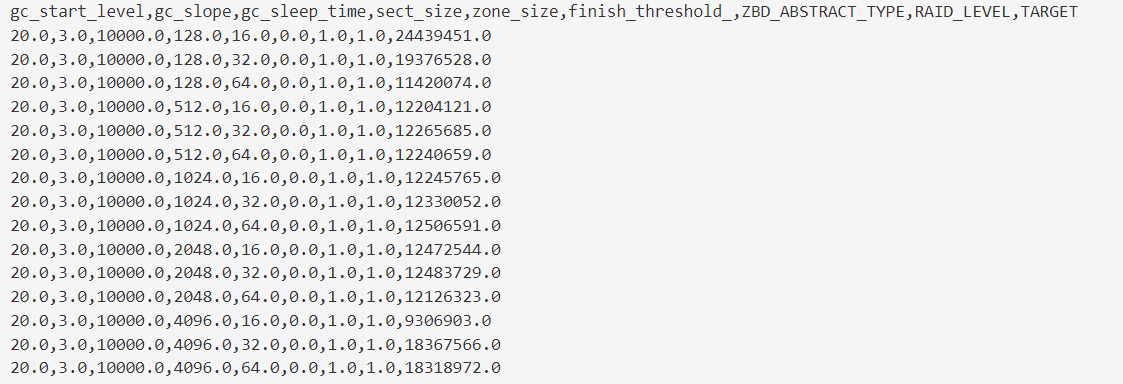
\includegraphics[width=0.85\textwidth]{fig/turnner1.png}
  \caption{ 调参测试数据 }
  \label{test-turnner1}
\end{figure}

设定参数进行AquaTuner的参数推荐流程,离散参数直接指定:

\begin{lstlisting}
SECT_SIZE_PARAM = 128
ZONE_SIZE_PARAM = 64
\end{lstlisting}

连续参数可以直接通过脚本defconfig获取。

接下来利用db\_bench进行参数跑分以及收集参数和目标值:

\begin{lstlisting}
  pre_throughput = 0
  now_throughput = 0
  for _ in range(1):
      sect_size = SECT_SIZE_PARAM
      zone_size = ZONE_SIZE_PARAM
      total_throughput = []
      for i in range(2):
          create_null_blk(sect_size, zone_size, 0, 64)
          os.system(CREATE_TMP_FILE)
          throughput_list = execute_adjust_param(2, sect_size, zone_size)
          total_throughput = total_throughput + throughput_list
          print("throughput list : {}".format(total_throughput))
          remove_null_blk()
      print("sect_size:{}".format(sect_size))
      print("zone_size:{}".format(zone_size))
      pre_throughput = now_throughput
      now_throughput = np.average(total_throughput)
\end{lstlisting}

代码的整体流程是,首先创建zone块,再在zone块上创建文件,得到跑分的吞吐量以及推荐参数,再将块zone块删除。

创建文件系统如下图所示,创建AquaFS的数据模块nullb0和作为log等文件存储的模块/tmp/aquafs。

\begin{lstlisting}
  CREATE_TMP_FILE = "mkdir -p /tmp/aquafs ;\
  sudo ../build/plugin/aquafs/aquafs mkfs --zbd nullb0 --aux-path /tmp/aquafs"
\end{lstlisting}

之后用db\_bench进行跑分,并进行智能调参模块的逻辑,按照指定推荐的离散参数跑一遍智能调参模块的结果如图 \ref{test-turnner2} 所示。

\begin{figure}[htbp]
  \centering
  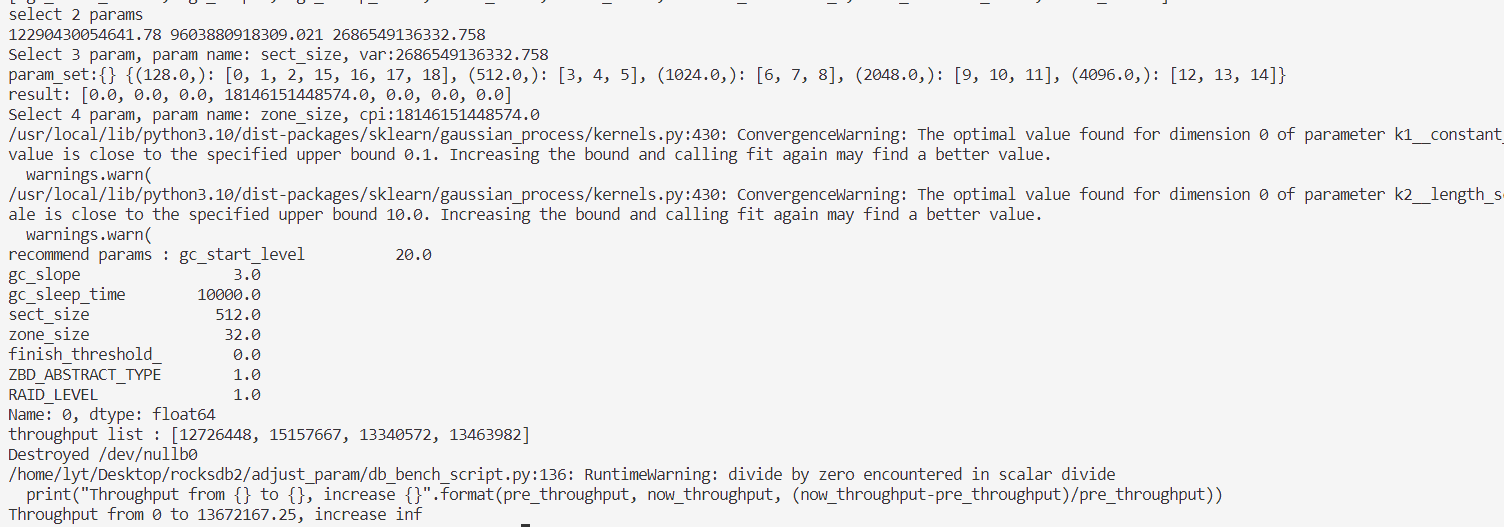
\includegraphics[width=0.85\textwidth]{fig/turnner2.png}
  \caption{ 调参测试过程 }
  \label{test-turnner2}
\end{figure}

在上图中推荐了两个参数,最重要的参数是sect\_size,其次是zone\_size,这符合现阶段的测试预期,因为我们的垃圾回收也就是gc还没有进行触发,,所以能够更改的参数现阶段只有块大小和zone\_size,而调参模块也根据现阶段的数据仓库中最优的参数进行了配置推荐。记录这里的平均吞吐量是13672167.25。

采用接下来的配置再进行测试:

\begin{lstlisting}
SECT_SIZE_PARAM = 512
ZONE_SIZE_PARAM = 32
\end{lstlisting}

最终结果如图 \ref{test-turnner3} 所示。

\begin{figure}[htbp]
  \centering
  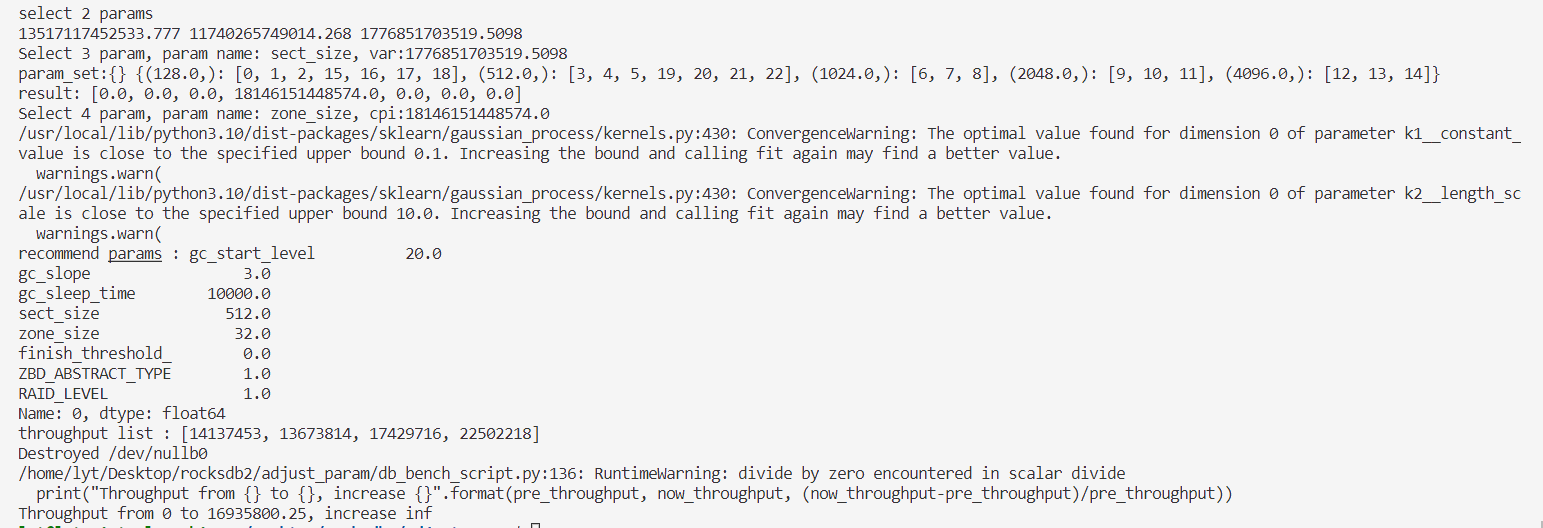
\includegraphics[width=0.85\textwidth]{fig/turnner3.png}
  \caption{ 调参测试结果 }
  \label{test-turnner3}
\end{figure}

平均吞吐量是16935800.25。相比于上一次的配置参数,吞吐量提升了23.87\%。

后续还将尝试测试触发gc来测试gc的参数,以及尝试融合文件系统后对整体的inode以及其他参数进行自动调整。


    \section{总结与展望}

\subsection{工作总结}

我们提出了 AquaFS,一个以 ZenFS 为原型的,基于 Zoned Namespace SSD 的高性能、高灵活性、高效,而且更加智能的适用于 Flash 存储介质的文件系统。

AquaFS 采用模块化设计,不同模块各司其职,分别负责不同的功能,使得 AquaFS 的功能更加清晰,易于维护和扩展。

在当前初赛阶段,我们实现了 AquaFS 的一些核心功能,包括:

\begin{itemize}
  \item 智能调参模块
  \begin{enumerate}
    \item 参照论文\cite{mahmud_confd_nodate},实现了高维度参数中重要参数筛选算法
    \item 针对当前轮获得的重要参数,实现了参数调整算法
  \end{enumerate}
  \item 智能动态分区 RAID
  \begin{enumerate}
    \item 实现了全盘 RAID 模式中的 RAID0、RAID1、RAID-C
    \item 分区 RAID 动态地址映射管理实现
    \item 分区 RAID 动态 RAID 逻辑实现
    \item 分区 RAID 数据块错误处理和数据恢复
  \end{enumerate}
  \item IO 加速实现:实现基于 Direct IO + io\_uring + C++协程 的高性能 IO 加速
  \item ExtFS 辅助文件系统
\end{itemize}

总体完成进度约 50\%。



\subsection{创新点和未来}

在初赛阶段,我们总结 AquaFS 的已经实现或者部分实现了的创新点主要有以下几点:

\begin{itemize}
  \item \textbf{更加智能}:ZenFS 许多逻辑都是固定的,而 AquaFS 通过智能调参、智能分类读写等方式提升其智能化水平。此外,AquaFS 还可以通过文件系统级冗余、文件系统读写分离、inode 缓存等方式提升其智能化水平。
  \item \textbf{更加安全}:ZenFS 在写入记录层面进行校验,但是对更常见的整块数据损坏无法有效应对,而 AquaFS 通过 RAID 等方式提升了针对 Zones 的数据安全性。
  \item \textbf{更加高效}:ZenFS 仅有 Direct IO 模式,而 AquaFS 支持 \verb|io_uring| 等更高效的异步 IO 模式。
\end{itemize}

在概述章节 \ref{overview} 中,我们总结了 AquaFS 相比于原型 ZenFS 的特点,其中还没有实现或者实现得还不够的创新点主要有以下几点:

\begin{itemize}
  \item \textbf{适用场景更广泛}:ZenFS 仅适用于软件特殊适配后的 ZNS 设备,而 AquaFS 可以通过融合文件系统和通用文件接口等方式适用于更多的软硬件设备。
  \item \textbf{更加灵活}:ZenFS 由于其简单而参数较少,且都由上层软件适配调整,而 AquaFS 可以通过调整参数、融合文件系统等方式提升其场景适用性,为没有软件适配的应用场景提供支持。
\end{itemize}

为了完成这些创新点,我们将在后续的比赛阶段继续努力,完成 AquaFS 的全部功能,包括:

\begin{itemize}
  \item 完善 AquaFS 的智能调参模块,针对垃圾回收、文件系统融合等算法进行调参
  \item 完善 Data Router,实现更加智能的数据路由,包括文件系统级冗余、文件系统读写分离、inode 缓存等
  \item 完善 AquaFS 的 IO 加速模块,实现 SPDK、xnvme 等用户态 NVMe 驱动的支持
  \item 完善 AquaFS 的 ExtFS 辅助文件系统,实现更加智能的文件系统融合
  \item 完善 AquaFS 的分区 RAID 功能,加强 RAID 分区分配逻辑的智能化
  \item 对更多的测试进行量化分析,分析并提升 AquaFS 的性能
  \item 争取获取到 ZNS SSD 设备,进行更加全面而更有说服力的测试和开发
\end{itemize}

虽然 AquaFS 在初赛阶段已经完成了部分工作,但是未来的工作仍然艰巨,还有许多问题需要解决:

\begin{itemize}
  \item \textbf{ZNS SSD 设备}:由于暂未申请到 ZNS SSD 设备,我们难以进行更加全面而更有说服力的测试和开发,这是迫切需要解决的问题。
  \item \textbf{鲁棒性}:在 AquaFS 当前已经发挥作用的模块中,许多代码都是初步实现,运行过程可能不稳定或存在隐形 Bug,还需要进一步完善,提升其鲁棒性。
  \item \textbf{量化评估}:对许多工作需要做性能和读写放大上的量化评估,包括智能调参模块、IO 加速模块、分区 RAID 等,这些评估需要大量的测试和分析,需要大量的时间和精力。
  \item \textbf{使用场景}:当前 AquaFS 能够适用的场景还不够广泛,只在 RocksDB 和以 RocksDB 为数据后端的 MySQL 中做了测试,需要进一步扩展其使用场景。
  \item \textbf{性能提升}:当前 AquaFS 的 IO 路径还是相对较长,一些 IO 请求过程还是过于复杂,需要用 Kernel bypass 的方式提升其性能。
\end{itemize}

总而言之,AquaFS 在初赛阶段已经完成了部分工作,但是还有许多工作需要完成,我们将在后续的比赛阶段继续努力,完成 AquaFS 的全部功能,提升其性能和鲁棒性,扩展其使用场景,为更多的应用场景提供支持。

% \begin{table}[htbp]
%   \centering
%   \caption{初赛进度情况}
%   \label{progress}
  \begin{tabular}{|l|l|p{8cm}|}
    \hline
    \textbf{改进内容}              & \textbf{完成进度} & \textbf{完成情况} \\
    \hline
    智能调参模块                   & 进度约70\%      & \checkmark 基于方差的重要参数选择方案 \\
                                  &                & \checkmark 基于高斯回归的调参方案 \\
                                  &                & $\square$ 将对垃圾回收参数进行进一步测试 \\
                                  &                & $\square$ 将对融合文件系统后的更多参数进行调优测试 \\
    \hline
    基于 Zone 的                  & 整体进度约 80\% & \checkmark 全盘 RAID 模式 RAID0、RAID1、RAID-C \\
    智能动态分区 RAID              &                & \checkmark 分区 RAID 模式 Zone 映射和 RAID 逻辑分配 \\
                                  &                & \checkmark 数据完整性检测和恢复 \\
    \hline
    异步 IO 优化                  & 进度约 60\%     & \checkmark 完成了 \verb|io_uring| 异步读写优化 \\
                                  &                & $\square$ 将进一步研究基于 spdk、xnvme 等的用户态 nvme 驱动 \\
    \hline
    融合通用文件系统               & 进度约 50\%     & \checkmark 基于 FUSE 和 Rust 完成一个 Ext2 兼容文件系统 \\
                                  &                & $\square$ 将进一步研究与 ZenFS 的结合方式 \\
                                  &                & $\square$ 将进一步研究智能数据请求分类方法 \\
    \hline
  \end{tabular}
% \end{table}
    %% APPENDIX
    \appendix
    \section{图表索引}
\subsection{图目录}
\subsection{表目录}
\newpage
\section{参考文献}
\printbibliography[heading=bibintoc]
\end{document}